%%%%%%%%%%%%%%%%%%%%%%%%%%%%%%%%%%%%%%%%%%%%%%%%%%%%%%%%%%%%%%%%%%%%%%%%%%%%%%%%
%2345678901234567890123456789012345678901234567890123456789012345678901234567890
%        1         2         3         4         5         6         7         8

\documentclass[letterpaper, 10 pt, conference]{ieeeconf}  % Comment this line out if you need a4paper

%\documentclass[a4paper, 10pt, conference]{ieeeconf}      % Use this line for a4 paper

%% \IEEEoverridecommandlockouts                              % This command is only needed if
                                                          % you want to use the \thanks command

\overrideIEEEmargins                                      % Needed to meet printer requirements.

% See the \addtolength command later in the file to balance the column lengths
% on the last page of the document

% The following packages can be found on http:\\www.ctan.org
%\usepackage{graphics} % for pdf, bitmapped graphics files
%\usepackage{epsfig} % for postscript graphics files
%\usepackage{mathptmx} % assumes new font selection scheme installed
%\usepackage{times} % assumes new font selection scheme installed
%\usepackage{amsmath} % assumes amsmath package installed
%\usepackage{amssymb}  % assumes amsmath package installed
\usepackage [vscale=0.76,includehead]{geometry}
\usepackage{graphicx}
\usepackage{amsmath}
\usepackage{array}
\usepackage{fullpage}
\usepackage{mathptmx} % font = times
\usepackage{helvet} % font sf = helvetica
\usepackage[latin1]{inputenc}
\usepackage{relsize}
\usepackage{graphicx}
\usepackage{caption}
\usepackage{subcaption}

\usepackage{pgfplots}
\newcommand{\rot}[2]{\ensuremath{C_{\,#1}^{\,#2}}}
\newcommand{\argmin}{\operatornamewithlimits{argmin}}
\definecolor{amethyst}{rgb}{0.5, 0.3, 0.7}

% and optionally (as of Pgfplots 1.3):
\pgfplotsset{compat=newest}
\pgfplotsset{plot coordinates/math parser=false}

\title{\LARGE \bf
Absolute scale velocity determination combining visual and inertial measurements for micro aerial vehicles
}


\author{Jacques Kaiser and Agostino Martinelli% <-this % stops a space
%% \thanks{*This work was not supported by any organization}% <-this % stops a space
%% \thanks{$^{1}$Albert Author is with Faculty of Electrical Engineering, Mathematics and Computer Science,
%%         University of Twente, 7500 AE Enschede, The Netherlands
%%         {\tt\small albert.author@papercept.net}}%
%% \thanks{$^{2}$Bernard D. Researcheris with the Department of Electrical Engineering, Wright State University,
%%         Dayton, OH 45435, USA
%%         {\tt\small b.d.researcher@ieee.org}}%
}


\begin{document}



\maketitle
\thispagestyle{empty}
\pagestyle{empty}


%%%%%%%%%%%%%%%%%%%%%%%%%%%%%%%%%%%%%%%%%%%%%%%%%%%%%%%%%%%%%%%%%%%%%%%%%%%%%%%%
\begin{abstract}

Hi

\end{abstract}


%%%%%%%%%%%%%%%%%%%%%%%%%%%%%%%%%%%%%%%%%%%%%%%%%%%%%%%%%%%%%%%%%%%%%%%%%%%%%%%%

\section{INTRODUCTION}




Autonomous mobile robots navigating in unknow environments have an intrinsic need to perform localization and mapping using only on-board sensors.
Concerning Micro Aerial Vehicles (MAV), a critical issue is to limit the number of on-board sensors to reduce weight and power consumption.
Therefore, a common setup is to combine a monocular camera with an inertial measurements unit (IMU).
On top of being cheap, these sensors have very interesting complementarities.
Additionaly, they can operate in indoor environments where Global Positioning System (GPS) signals are shadowed.
An open question is how to optimally fuse the information provided by these sensors.

Currently, most sensor fusion algorithms are either filter based or iterative. That is, given a current state and measurements, they return an updated state.
While working well in practice, these algorithms need to be provided by an external initial state.

The initialization of a filter based method is critical.
Due to nonlinearities of the system, a poor initialization can result into converging towards local minima and  providing faulty states with high confidence.
Indeed, another shortcoming of filters is that they can silently fail.

In this work we demonstrate the efficiency of a recent closed-form solution introduced in \cite{Martinelli2012}\cite{Martinelli2014} that fuses visual and inertial data to obtain the structure of the environment at the global scale along with the attitude and the speed of the robot.

By nature, a closed-form solution is deterministic and thus does not require any initialization.
It is assumed that the camera is calibrated and the transformation between the IMU and the camera is known.
This is a fair assumption for industrial drones to come pre-calibrated.

In this work, we have studied the recent closed-form solution proposed by \cite{Martinelli2014} that performs visual-inertial sensor fusion without requiring an initialization.
We implemented this method in order to test it with real terrain data.
This allowed us to identify its bottlenecks and bring modifications to overcome them.

Specifically, we started by reformulating the equations for greater numerical stability.
This lead to a major leap in the quality of the estimations.

We then investigated the impact of biased inertial measurements.
Despite the case of biased accelerometer was originally studied in \cite{Martinelli2014} we show that its low impact on the system makes it hard to estimate.

One major bottleneck of this method was the impact of biased gyroscope measurements.
In other words, the performance becomes very poor in presence of a bias on the gyroscope and, in practice, the overall method could only be successfully used with a very precise - and expensive - gyroscope.
We then introduced a simple method that automatically estimates this bias.

However, this method requires a significant amount of data to provide correct estimates of the gyroscope bias (either many features or long time of integration).
We were able to get rid of this limitation with a simple statistical trick by adding a regularization term to our cost function.
%tweak in the cost function we are minimizing.

By adding this new method for the bias estimation to the original method we obtain results which are equivalent to the ones in absence of bias.
Compared to the original method, the new method is now robust to the gyroscope bias, and also provides the gyroscope bias.
%% Specifically, this method can accurately estimate the initial speed, the gravity, the distance to the features and the gyroscope bias for very short time of integration (around 2 seconds) and low amount of observed point features (around 5).


%% \begin{figure}[h!]
%%         \centering
%%    \resizebox{0.4\textwidth}{!}{\input{./graph}}
%%         \caption{Estimation error of the original formulation of the Closed-Form solution against the improved Closed-Form solution observing 7 features over 3 seconds.}
%% \end{figure}

\section{RELATED WORK}
\section{THE CLOSED-FORM SOLUTION}

In this paper, we do not provide a new derivation of the closed-form solution.
Instead, we consider the latest derivation proposed in \cite{Martinelli2014}.
Specifically, the author expresses the state of the MAV with respect to the visual and inertial measurements in Equation \ref{eq:final1}:


\begin{equation} \tag{6} \label{eq:final1}
S_j = \lambda_1^i\mu_1^i - V t_j - G \frac{t_j^2}{2} - \lambda^i_j \mu^i_j
\end{equation}
With:
\begin{itemize}
\item $\mu_j^i$ the normalized bearing of point feature $i$ at time $t_j$ in the initial local frame;
\item $\lambda_j^i$ the distance to the point feature $i$ at time $t_j$;
\item $V$ the initial velocity in the initial local frame;
\item $G$ the initial gravity in the initial local frame;
\item $S_j$ the integration up to time $t_j$ of the rotated linear acceleration data.
\end{itemize}

\begin{figure}[h!]
  \centering
  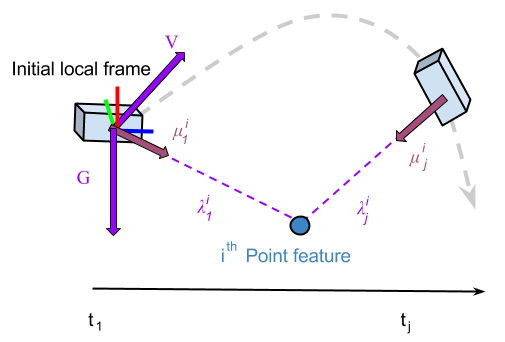
\includegraphics[width=0.90\columnwidth]{images/closedFormExplained}
  \caption{Visual representation of Equation \ref{eq:final1}.
  The unknowns of the equation are colored in \textcolor{amethyst}{purple}.}
\end{figure}


The unknowns of Equation \ref{eq:final1} are the distances $\lambda_j^i$ and the vectors $V$ and $G$.
Note that the knowledge of $G$ is equivalent to the knowledge of the roll and pitch angles.
The vectors $\mu_j^i$ are fully determined by camera observations and gyroscope measurements,
and the vectors $S_j$ are determined by accelerometer and gyroscope measurements.

As Equation \ref{eq:final1} holds for each three dimensions of all point features $i=1,...,N$ and each observation starting from the second one $j=2,...n_i$, we therefore have a system consisting of $3(n_i-1)N$ equations in $6 + Nn_i$ unknowns.
Indeed, note that when the first observation occurs, at $t_j = 0$, Equation \ref{eq:final1} is always satisfied thus does not provide information.
We can write our system using matrix formulation.
Solving the system is equivalent to inverting a matrix of $3(n_i-1)N$ rows and $6+Nn_i$ columns.

In \cite{Martinelli2014}, the author proceeded to one more step before expressing the underlying linear system.
For an observation at time $t_j$, the equation of the first point feature $i=1$ happening at time $t_j$ is subtracted to all other point features $1<i<=N$ at time $t_j$ (Equation 7).
This additional step has the effect to corrupt all measurements with the first measurement,
hence worsening the performance of the closed-form solution.
In this paper, we do not take to this additional step.

The linear system in Equation \ref{eq:final1} can be written in the following compact format:

\begin{equation}
\label{eq:mat1} \tag{9}
\Xi X = S
\end{equation}

The matrix $\Xi$ and the vector $S$ are fully determined by the measurements, while $X$ is the unknown vector.
We have:

\[
S \equiv [S_2^T, ...,S_2^T, S_3^T,...,S_3^T,...,S_{n_i}^T,...,S_{n_i}^T]^T
\]
\[
X \equiv [ G^T, V^T, \lambda_1^1, ..., \lambda_1^N, ..., \lambda_{n_i}^1, ..., \lambda_{n_i}^N]^T \\
\]

\begin{multline}
  \Xi \equiv \\
  \left[
    {\scriptscriptstyle
    \begin{array}{l|l|l|l|l|l|l|l|l|l|l}
      T_2 & S_2 & \mu_1^1 & 0_3 & 0_3 & -\mu_2^1 & 0_3 & 0_3 & 0_3 & 0_3 & 0_3 \\
      T_2 & S_2 & 0_3 & \mu_1^2 & 0_3 & 0_3 & -\mu_2^2 & 0_3 & 0_3 & 0_3 & 0_3 \\
      ... & ... & ... & ... & ... & ... & ... & ... & ... & ... & ... \\
      T_2 & S_2 & 0_3 & 0_3 & \mu_1^N & 0_3 & 0_3 & -\mu_2^N & 0_3 & 0_3 & 0_3 \\
      ... & ... & ... & ... & ... & ... & ... & ... & ... & ... & ... \\
      ... & ... & ... & ... & ... & ... & ... & ... & ... & ... & ... \\
      T_{n_i} & S_{n_i} & \mu_1^1 & 0_3 & 0_3 & 0_3 & 0_3 & 0_3 & -\mu_{n_i}^1 & 0_3 & 0_3 \\
      T_{n_i} & S_{n_i} & 0_3 & \mu_1^2 & 0_3 & 0_3 & 0_3 & 0_3 & 0_3 & -\mu_{n_i}^2 & 0_3 \\
      ... & ... & ... & ... & ... & ... & ... & ... & ... & ... & ... \\
      T_{n_i} & S_{n_i} & 0_3 & 0_3 & \mu_1^N & 0_3 & 0_3 & 0_3 & 0_3 & 0_3 & -\mu_{n_i}^N
    \end{array}
    }
    \right]
\end{multline}

Where $T_j \equiv - \frac{t^2_j}{2} I_3$, $S_j \equiv -t_j I_3$ and $I_3$ is the identity 3 x 3 matrix; $0_{33}$ is the 3 x 3 zero matrix.
Note that the matrix $\Xi$ and the vector $S$ are slightly different from the one proposed in \cite{Martinelli2014}.
This is due to the additional step we did not take for numerical stability reasons.

The sensor information is completely contained in the above linear system. Additionally, in \cite{Martinelli2014}, the author added a quadratic equation assuming the gravitational acceleration is a priori known.
Let us denote the gravitational magnitude by $g$.
We have the extra constraint $|G| = g$. We can express this constraint in matrix formulation:

\begin{equation}
\label{eq:mat2} \tag{10}
| \Pi X | ^2 = g^2
\end{equation}

With $\Pi \equiv [I_3, 0_3, ..., 0_3]$.

We can therefore recover the initial velocity, the roll and pitch angles and the distances to the point features
by finding the vector $X$ which satisfies \ref{eq:mat1} and \ref{eq:mat2}.

In the next sections, we will evaluate the performance of this method on real terrain data.
This will allow us to identify its weaknesses and bring modifications to overcome them.

%% The system therefore becomes:

%% \begin{equation} \label{eq:final2}
%% \left[
%% \begin{array}{lcl}
%% S_j &=& \lambda_1^i\mu_1^i - V t_j - G \frac{t_j^2}{2} - \lambda^i_j \mu^i_j\\
%% 0_3 &=& \lambda_1^1\mu_1^1 - \lambda_j^1\mu_j^1 - \lambda_1^i\mu_1^i + \lambda^i_j \mu^i_j
%% \end{array}
%% \right.
%% \end{equation}



\section{PERFORMANCE BOTTLENECKS}

\subsection{Test setup}

The MAV performs a motion while being tracked with an optical Vicon system.
We can therefore compare our estimations with the ground truth.
We define the relative error as the euclidian distance between the estimation and the ground truth,
normalized by the groud truth.
We measure our error on the absolute scale by computing the mean error over all estimated distances to point features $\lambda_j^i$.

To identify the performance bottlenecks, we used IMU data obtained from terrain acquisitions
while we simulated the point feature observations.
This separation allowed us to know the ground truth for the distance to the point features
and also better understand the weaknesses of our method.

We represent this setup in Fig. \ref{fig:testsetup}.

\begin{figure}[h!]
  \centering
  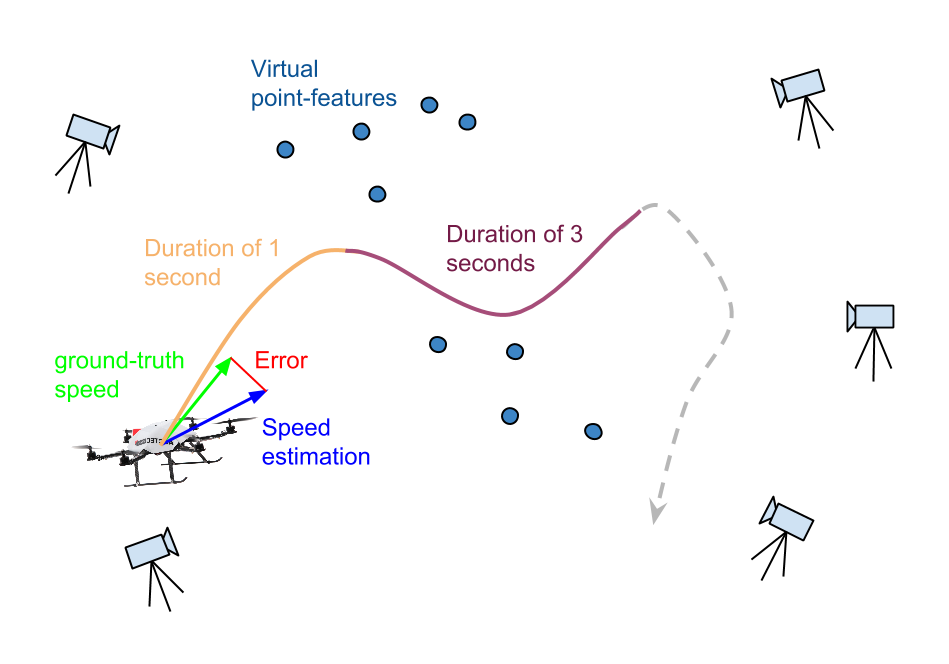
\includegraphics[width=\columnwidth]{images/setupTestDroneError.png}
  \caption{Test setup for identifying the performance bottlenecks.
    The drone is equipped with an IMU, and the visual measurements are simulated.
    It performs a motion while being tracked by a Vicon system.\label{fig:testsetup}}
\end{figure}

In general, we use one camera observation every 0.3 seconds, even if the camera provides significantly more frames.
Indeed, we can discard most of the camera observations.
If two observations are too close to each other, then the additional equations do not bring much information to our system.
Reducing the number of considered frames reduces the size of the matrices, thus speeds up the computations.

As an example, over a time interval of 3 seconds, we obtain $11$ distinct frames.
When observing 7 features, it yields a system of $3\times 10\times 7 = 210$ equations and $6+7\times 10=76$ unknowns.

The method we use to solve the overconstrained linear system $\Xi X = S$ is a singular value decomposition (SVD) since it yields numerically robust solutions.

In this section, we will start by presenting the results obtained with the original closed-form solution on terrain IMU data.
Our goal is to identify its performance bottlenecks and introduce modifications to overcome them.

%% The case of a biased gyroscope is addressed in chapter \ref{ch:gyro}.
%% Indeed, the main contribution of this report is the simple method introduced in Section \ref{sec:computeBias} to compute the gyroscope bias with the closed-form solution, which happened to be a major performance bottleneck.

\subsection{Original closed-form solution performance}

The original closed-form solution described in Equation \ref{eq:mat1} will be used as a basis for our work.
Moreover, we can also use the knowledge of the gravity magnitude in order to refine our results with Equation \ref{eq:mat2}.
In this case, we are minimizing a linear objective function with a quadratic constraint.
in Fig. \ref{fig:original}, we represent the quality of the evaluations with and without this additional constraint.


\begin{figure}[h!]
  \centering
    \resizebox{0.6\columnwidth}{!}{% This file was created by matlab2tikz.
% Minimal pgfplots version: 1.3
%
%The latest updates can be retrieved from
%  http://www.mathworks.com/matlabcentral/fileexchange/22022-matlab2tikz
%where you can also make suggestions and rate matlab2tikz.
%
\definecolor{mycolor1}{rgb}{0.00000,0.44700,0.74100}%
%
\begin{tikzpicture}[%
arrow1/.style={->,color=mycolor1,solid}
]

\begin{axis}[%
width=3in,
height=4in,
at={(4.349344in,1.108021in)},
scale only axis,
xmin=-2.32898813721698,
xmax=0.977364285688564,
tick align=outside,
xmajorgrids,
ymin=-2.9032427347286,
ymax=2.44018172608593,
ymajorgrids,
zmin=-2.69119678019502,
zmax=3.37775853360063,
zmajorgrids,
view={-10.5}{30},
axis x line*=bottom,
axis y line*=left,
axis z line*=left
]
\addplot3 [arrow1] coordinates{(-0.835478573784258,-1.04332852496064,1.41382166234386) (-0.782352063146176,-1.04279555272648,1.41387893962832)};
\addplot3 [arrow1] coordinates{(-0.714209573958594,-0.974408019658836,1.43092404685403) (-0.661137392310022,-0.974064033076341,1.43336098775606)};
\addplot3 [arrow1] coordinates{(-0.600531605535264,-0.896122809173835,1.44450216358562) (-0.547477370190682,-0.895726941673801,1.44729588397106)};
\addplot3 [arrow1] coordinates{(-0.500901254122354,-0.81485572464222,1.45500787211561) (-0.4478851064577,-0.814744379320697,1.45847040900161)};
\addplot3 [arrow1] coordinates{(-0.404829455976097,-0.721113285032798,1.46331325446157) (-0.351938461913981,-0.721397621406281,1.468330761075)};
\addplot3 [arrow1] coordinates{(-0.320204251822945,-0.618787705110875,1.46900301057783) (-0.267503559956665,-0.619016376936769,1.47573340868488)};
\addplot3 [arrow1] coordinates{(-0.252381220672505,-0.51603340292696,1.47243003206791) (-0.199753908159354,-0.516292519346331,1.47971098729317)};
\addplot3 [arrow1] coordinates{(-0.194479455243222,-0.401511229652653,1.47488651276691) (-0.14204662534326,-0.402154655682573,1.48343623932942)};
\addplot3 [arrow1] coordinates{(-0.152418688253173,-0.28104011784627,1.47558779075496) (-0.100159193213691,-0.281671539015199,1.4851407985637)};
\addplot3 [arrow1] coordinates{(-0.125767731567136,-0.156144502380668,1.47494403192677) (-0.0735979636932584,-0.156998296352248,1.48495901213183)};
\addplot3 [arrow1] coordinates{(-0.116249088788111,-0.0371709603012026,1.47518123428233) (-0.0641952399993195,-0.0382287915196861,1.48576382810685)};
\addplot3 [arrow1] coordinates{(-0.122282880399225,0.0894040630904905,1.47517738581066) (-0.0704412471556641,0.0882159662419642,1.48674228793678)};
\addplot3 [arrow1] coordinates{(-0.145053367682376,0.2149684597659,1.47419910983079) (-0.0930986075573921,0.213833016707382,1.48525022480097)};
\addplot3 [arrow1] coordinates{(-0.181116568724285,0.33042271421565,1.47354868510755) (-0.12915874363247,0.329241360705766,1.48458056111669)};
\addplot3 [arrow1] coordinates{(-0.234252184869997,0.446932038350022,1.47276016252391) (-0.182113213604754,0.445972501318801,1.48292482861561)};
\addplot3 [arrow1] coordinates{(-0.300393565705767,0.555603954889073,1.47232434430534) (-0.248130908736752,0.554834689074976,1.48184990934445)};
\addplot3 [arrow1] coordinates{(-0.373298719383221,0.648922576388966,1.47132963925705) (-0.32098613083632,0.648845650277542,1.48060868201824)};
\addplot3 [arrow1] coordinates{(-0.461892630028163,0.733403249851481,1.47112099631838) (-0.409568880231268,0.733469314309986,1.48033697783676)};
\addplot3 [arrow1] coordinates{(-0.559275389855508,0.803645100931922,1.46896971956663) (-0.506836993733445,0.804632974883657,1.47745218323404)};
\addplot3 [arrow1] coordinates{(-0.660628367565958,0.85340016810821,1.46855988145047) (-0.608078629013239,0.854474569314938,1.4763112756964)};
\addplot3 [arrow1] coordinates{(-0.77324887413896,0.891136239024197,1.46746019576887) (-0.720471921745042,0.892942955504477,1.47329479466152)};
\addplot3 [arrow1] coordinates{(-0.891299934790413,0.911314987685633,1.46809495935247) (-0.83849505216681,0.913442400435598,1.47355682339021)};
\addplot3 [arrow1] coordinates{(-1.0111290553568,0.915240872265903,1.468598090367) (-0.958189213650306,0.918038224821616,1.47209972590463)};
\addplot3 [arrow1] coordinates{(-1.12571940848728,0.903758649927526,1.46961661022113) (-1.07269938379418,0.90636515524614,1.47180672077438)};
\addplot3 [arrow1] coordinates{(-1.24553603250621,0.875984582695998,1.47154962607067) (-1.1924489292668,0.877876610517143,1.47249470439564)};
\addplot3 [arrow1] coordinates{(-1.3607816013423,0.835339171287469,1.47218746030471) (-1.30772452051326,0.837565935767234,1.47054393770992)};
\addplot3 [arrow1] coordinates{(-1.46419344786626,0.782575971991294,1.47339785704681) (-1.41114194999108,0.784205044908038,1.47103181239383)};
\addplot3 [arrow1] coordinates{(-1.56472291422273,0.713719456160076,1.47405951493983) (-1.51175276992938,0.715104981532175,1.4701920085529)};
\addplot3 [arrow1] coordinates{(-1.65576204418145,0.63074719555968,1.47532915292966) (-1.60290479125813,0.631143829882531,1.46997499872177)};
\addplot3 [arrow1] coordinates{(-1.73132783061723,0.544003042604293,1.47492183268681) (-1.67878893401333,0.544396897059298,1.46703369634288)};
\addplot3 [arrow1] coordinates{(-1.79740232936522,0.444033710191173,1.47635547853074) (-1.74491242862433,0.443618340058418,1.46814869715605)};
\addplot3 [arrow1] coordinates{(-1.84890070462009,0.336896487686537,1.47719055096603) (-1.79655107094903,0.335915727029584,1.46817570567021)};
\addplot3 [arrow1] coordinates{(-1.8856494738633,0.224673403378243,1.47696396107085) (-1.83356035855119,0.223197896940006,1.4666073004401)};
\addplot3 [arrow1] coordinates{(-1.90483141348729,0.11403315139582,1.47654172161289) (-1.85280810168368,0.112090842184906,1.46593436866407)};
\addplot3 [arrow1] coordinates{(-1.90991827668782,-0.00476480483644565,1.47622526122602) (-1.85789670210118,-0.00720057800866189,1.46571163867011)};
\addplot3 [arrow1] coordinates{(-1.8982083285231,-0.123105386309713,1.47622070709117) (-1.84636044018161,-0.125429394408634,1.46485809587932)};
\addplot3 [arrow1] coordinates{(-1.87222375253455,-0.233038005434342,1.47472267151996) (-1.82022817329984,-0.235345576970085,1.46405269840276)};
\addplot3 [arrow1] coordinates{(-1.82971610124117,-0.346387807548545,1.47408407293631) (-1.77762542487408,-0.348575984286811,1.46386219488729)};
\addplot3 [arrow1] coordinates{(-1.7731666142271,-0.453272885967697,1.47269553121087) (-1.72106023695358,-0.455020994521588,1.4624689464153)};
\addplot3 [arrow1] coordinates{(-1.7031619738735,-0.552976340403652,1.47144825129321) (-1.65096502426862,-0.554194019310345,1.4616141685859)};
\addplot3 [arrow1] coordinates{(-1.62566192563085,-0.63829012238084,1.47034716728465) (-1.57345267063604,-0.639186731181834,1.46054394035606)};
\addplot3 [arrow1] coordinates{(-1.53259324250719,-0.716868801295633,1.46963979295776) (-1.48017344643549,-0.71725066243648,1.46099498905372)};
\addplot3 [arrow1] coordinates{(-1.43017642763263,-0.781814333373981,1.46995872414126) (-1.37750354270295,-0.781572050422345,1.46301452045596)};
\addplot3 [arrow1] coordinates{(-1.32689048225905,-0.82921409690145,1.47063735140649) (-1.2742467660064,-0.828706484475863,1.46348927884084)};
\addplot3 [arrow1] coordinates{(-1.21142274060827,-0.863860620630827,1.47141608951282) (-1.15869373216687,-0.862787904327957,1.46499624362771)};
\addplot3 [arrow1] coordinates{(-1.09146691329025,-0.881864584778972,1.47288226944595) (-1.03860370362738,-0.88025976690567,1.46782073841264)};
\addplot3 [arrow1] coordinates{(-0.976106737126645,-0.883140532358599,1.47383096453613) (-0.923117664834161,-0.88109054503773,1.47056458393459)};
\addplot3 [arrow1] coordinates{(-0.854133474214521,-0.867094916759381,1.47498900445891) (-0.801088148149646,-0.864410589497775,1.4736846875911)};
\addplot3 [arrow1] coordinates{(-0.735872481283784,-0.835929216965365,1.47631792889777) (-0.682809402677152,-0.833279148824848,1.47630059958849)};
\addplot3 [arrow1] coordinates{(-0.622591783264491,-0.788766680097929,1.4776086265601) (-0.569544608559794,-0.786248822966117,1.47914847200075)};
\addplot3 [arrow1] coordinates{(-0.5230922921375,-0.729888321755682,1.4784055922169) (-0.47012933271689,-0.727350975077879,1.48175227324673)};
\addplot3 [arrow1] coordinates{(-0.426910637124303,-0.654562633651572,1.47937440637353) (-0.374008390350352,-0.652460636386582,1.48380694136312)};
\addplot3 [arrow1] coordinates{(-0.342326575468263,-0.566454232612501,1.47926269428178) (-0.289503914229201,-0.564644317077975,1.48466677959283)};
\addplot3 [arrow1] coordinates{(-0.273133035490774,-0.473644467240719,1.47927853625887) (-0.220396275332261,-0.472153410797879,1.48554944937705)};
\addplot3 [arrow1] coordinates{(-0.213107244857738,-0.366695363648817,1.47911772965251) (-0.160535001069963,-0.365611126236492,1.48671358938137)};
\addplot3 [arrow1] coordinates{(-0.16781778102554,-0.253322621000146,1.47906502261259) (-0.115452416317831,-0.252755314583471,1.48802382918077)};
\addplot3 [arrow1] coordinates{(-0.13977310739712,-0.141336212570664,1.47862052006325) (-0.0874829984252,-0.14112148560748,1.48802327863209)};
\addplot3 [arrow1] coordinates{(-0.124961152245377,-0.0206067152854782,1.47811746037667) (-0.0727797330706261,-0.0208017048708022,1.48810620127022)};
\addplot3 [arrow1] coordinates{(-0.835478573784258,-1.04332852496064,1.41382166234386) (-0.8359989523433,-0.990687294702958,1.40665622057233)};
\addplot3 [arrow1] coordinates{(-0.714209573958594,-0.974408019658836,1.43092404685403) (-0.71424027529558,-0.921711875804426,1.42415433836909)};
\addplot3 [arrow1] coordinates{(-0.600531605535264,-0.896122809173835,1.44450216358562) (-0.60055274065995,-0.843464796655706,1.4374419409535)};
\addplot3 [arrow1] coordinates{(-0.500901254122354,-0.81485572464222,1.45500787211561) (-0.500516729861083,-0.762271210940679,1.44742931469794)};
\addplot3 [arrow1] coordinates{(-0.404829455976097,-0.721113285032798,1.46331325446157) (-0.403845392939075,-0.668510066958503,1.45592092459642)};
\addplot3 [arrow1] coordinates{(-0.320204251822945,-0.618787705110875,1.46900301057783) (-0.31910304224293,-0.56611123240852,1.46216999998462)};
\addplot3 [arrow1] coordinates{(-0.252381220672505,-0.51603340292696,1.47243003206791) (-0.251330546580928,-0.463222899876944,1.46671511087638)};
\addplot3 [arrow1] coordinates{(-0.194479455243222,-0.401511229652653,1.47488651276691) (-0.192840092727392,-0.348756930831475,1.46880293494662)};
\addplot3 [arrow1] coordinates{(-0.152418688253173,-0.28104011784627,1.47558779075496) (-0.150755626623864,-0.228233825488809,1.46998036833968)};
\addplot3 [arrow1] coordinates{(-0.125767731567136,-0.156144502380668,1.47494403192677) (-0.12424089333417,-0.103148472930448,1.47150846789888)};
\addplot3 [arrow1] coordinates{(-0.116249088788111,-0.0371709603012026,1.47518123428233) (-0.114615551948374,0.0158627186918971,1.47244738671562)};
\addplot3 [arrow1] coordinates{(-0.122282880399225,0.0894040630904905,1.47517738581066) (-0.120536667790788,0.142451300178024,1.47279939262877)};
\addplot3 [arrow1] coordinates{(-0.145053367682376,0.2149684597659,1.47419910983079) (-0.143985693885372,0.26808513995113,1.47463709548254)};
\addplot3 [arrow1] coordinates{(-0.181116568724285,0.33042271421565,1.47354868510755) (-0.180272264207056,0.383517716239467,1.47525789037347)};
\addplot3 [arrow1] coordinates{(-0.234252184869997,0.446932038350022,1.47276016252391) (-0.233828015050327,0.499984008489245,1.47559247906326)};
\addplot3 [arrow1] coordinates{(-0.300393565705767,0.555603954889073,1.47232434430534) (-0.300552982439863,0.608483216027342,1.47746941966374)};
\addplot3 [arrow1] coordinates{(-0.373298719383221,0.648922576388966,1.47132963925705) (-0.374497865279204,0.701548450770545,1.4785263654129)};
\addplot3 [arrow1] coordinates{(-0.461892630028163,0.733403249851481,1.47112099631838) (-0.463390609738487,0.785885589472828,1.47924956060274)};
\addplot3 [arrow1] coordinates{(-0.559275389855508,0.803645100931922,1.46896971956663) (-0.561779749935731,0.855876320092012,1.4783687300628)};
\addplot3 [arrow1] coordinates{(-0.660628367565958,0.85340016810821,1.46855988145047) (-0.663096041651499,0.905616355805873,1.47805165681643)};
\addplot3 [arrow1] coordinates{(-0.77324887413896,0.891136239024197,1.46746019576887) (-0.776162654365532,0.943188104490355,1.47769868486406)};
\addplot3 [arrow1] coordinates{(-0.891299934790413,0.911314987685633,1.46809495935247) (-0.894483205008447,0.963292845747602,1.47862503697216)};
\addplot3 [arrow1] coordinates{(-1.0111290553568,0.915240872265903,1.468598090367) (-1.01457262373411,0.967196913042023,1.47915390091706)};
\addplot3 [arrow1] coordinates{(-1.12571940848728,0.903758649927526,1.46961661022113) (-1.12870673650547,0.955770482010431,1.48003575929192)};
\addplot3 [arrow1] coordinates{(-1.24553603250621,0.875984582695998,1.47154962607067) (-1.24757760890174,0.92802783911803,1.4820398548327)};
\addplot3 [arrow1] coordinates{(-1.3607816013423,0.835339171287469,1.47218746030471) (-1.36262304853926,0.887295586985071,1.48313521864817)};
\addplot3 [arrow1] coordinates{(-1.46419344786626,0.782575971991294,1.47339785704681) (-1.46529282137377,0.834518260130555,1.48451107230689)};
\addplot3 [arrow1] coordinates{(-1.56472291422273,0.713719456160076,1.47405951493983) (-1.5652568967769,0.765633671435224,1.4853441322424)};
\addplot3 [arrow1] coordinates{(-1.65576204418145,0.63074719555968,1.47532915292966) (-1.6551505893238,0.682941744921819,1.48523211271491)};
\addplot3 [arrow1] coordinates{(-1.73132783061723,0.544003042604293,1.47492183268681) (-1.73046696762054,0.59646442785001,1.48327500248451)};
\addplot3 [arrow1] coordinates{(-1.79740232936522,0.444033710191173,1.47635547853074) (-1.79571325702715,0.49650733889646,1.48450279697329)};
\addplot3 [arrow1] coordinates{(-1.84890070462009,0.336896487686537,1.47719055096603) (-1.84662989986242,0.38944900285515,1.48465982588888)};
\addplot3 [arrow1] coordinates{(-1.8856494738633,0.224673403378243,1.47696396107085) (-1.88281845712898,0.277297087282515,1.48370537852278)};
\addplot3 [arrow1] coordinates{(-1.90483141348729,0.11403315139582,1.47654172161289) (-1.90186703311565,0.16685592004337,1.4814080378878)};
\addplot3 [arrow1] coordinates{(-1.90991827668782,-0.00476480483644565,1.47622526122602) (-1.9069474309929,0.0482259163666367,1.47864827895235)};
\addplot3 [arrow1] coordinates{(-1.8982083285231,-0.123105386309713,1.47622070709117) (-1.89525969718442,-0.0701227028164296,1.47883877808849)};
\addplot3 [arrow1] coordinates{(-1.87222375253455,-0.233038005434342,1.47472267151996) (-1.86966578736339,-0.179979645961832,1.47571301334828)};
\addplot3 [arrow1] coordinates{(-1.82971610124117,-0.346387807548545,1.47408407293631) (-1.82769587498613,-0.293307752537922,1.47301640322356)};
\addplot3 [arrow1] coordinates{(-1.7731666142271,-0.453272885967697,1.47269553121087) (-1.77172351336644,-0.400191158467165,1.47097473542601)};
\addplot3 [arrow1] coordinates{(-1.7031619738735,-0.552976340403652,1.47144825129321) (-1.70252220948049,-0.499945678834757,1.46827758767898)};
\addplot3 [arrow1] coordinates{(-1.62566192563085,-0.63829012238084,1.47034716728465) (-1.62578781547862,-0.585446874924746,1.46484363907919)};
\addplot3 [arrow1] coordinates{(-1.53259324250719,-0.716868801295633,1.46963979295776) (-1.53328554657647,-0.664146558298759,1.46311298047982)};
\addplot3 [arrow1] coordinates{(-1.43017642763263,-0.781814333373981,1.46995872414126) (-1.43139414793788,-0.729217294199575,1.46255723104782)};
\addplot3 [arrow1] coordinates{(-1.32689048225905,-0.82921409690145,1.47063735140649) (-1.32856655220397,-0.776816091920849,1.4620145133435)};
\addplot3 [arrow1] coordinates{(-1.21142274060827,-0.863860620630827,1.47141608951282) (-1.21361781028346,-0.811597090576828,1.4621199307317)};
\addplot3 [arrow1] coordinates{(-1.09146691329025,-0.881864584778972,1.47288226944595) (-1.09402231915119,-0.829781531333792,1.46270686196614)};
\addplot3 [arrow1] coordinates{(-0.976106737126645,-0.883140532358599,1.47383096453613) (-0.978747975276547,-0.831058980742426,1.46366979752858)};
\addplot3 [arrow1] coordinates{(-0.854133474214521,-0.867094916759381,1.47498900445891) (-0.857011323150831,-0.814937652784797,1.46529100090905)};
\addplot3 [arrow1] coordinates{(-0.735872481283784,-0.835929216965365,1.47631792889777) (-0.738476628438728,-0.783852290601861,1.466123536773)};
\addplot3 [arrow1] coordinates{(-0.622591783264491,-0.788766680097929,1.4776086265601) (-0.624739926962338,-0.736819840049625,1.4666713160901)};
\addplot3 [arrow1] coordinates{(-0.5230922921375,-0.729888321755682,1.4784055922169) (-0.524971715888277,-0.677708080877601,1.46858705358131)};
\addplot3 [arrow1] coordinates{(-0.426910637124303,-0.654562633651572,1.47937440637353) (-0.428193392022673,-0.602300685244502,1.46990040187514)};
\addplot3 [arrow1] coordinates{(-0.342326575468263,-0.566454232612501,1.47926269428178) (-0.343238917398763,-0.514039654626296,1.47062596345364)};
\addplot3 [arrow1] coordinates{(-0.273133035490774,-0.473644467240719,1.47927853625887) (-0.273763776290894,-0.42101060571886,1.47206797039974)};
\addplot3 [arrow1] coordinates{(-0.213107244857738,-0.366695363648817,1.47911772965251) (-0.21331751288098,-0.313915437008706,1.47303919332451)};
\addplot3 [arrow1] coordinates{(-0.16781778102554,-0.253322621000146,1.47906502261259) (-0.167414187006479,-0.200502014072416,1.47336115828022)};
\addplot3 [arrow1] coordinates{(-0.13977310739712,-0.141336212570664,1.47862052006325) (-0.139223893072342,-0.0883811959786041,1.47435694714513)};
\addplot3 [arrow1] coordinates{(-0.124961152245377,-0.0206067152854782,1.47811746037667) (-0.124317749360381,0.0324676991129846,1.47579237077501)};
\addplot3 [arrow1] coordinates{(-0.797432085550432,-1.04564433889453,1.39404536999931) (-0.797560717758648,-1.03847982284503,1.44668914110473)};
\addplot3 [arrow1] coordinates{(-0.676163085724768,-0.976723833592727,1.41114775450949) (-0.678623993109622,-0.969962800478305,1.46378752881312)};
\addplot3 [arrow1] coordinates{(-0.562485117301438,-0.898438623107725,1.42472587124107) (-0.565306666162641,-0.89138947569609,1.47730972670509)};
\addplot3 [arrow1] coordinates{(-0.462854765888528,-0.81717153857611,1.43523157977106) (-0.466297686241963,-0.809584049290465,1.48770337961105)};
\addplot3 [arrow1] coordinates{(-0.366782967742272,-0.723429098966689,1.44353696211702) (-0.371711237187859,-0.715976980226169,1.49590958434674)};
\addplot3 [arrow1] coordinates{(-0.282157763589119,-0.621103519044765,1.44922671823328) (-0.288801398659188,-0.614186120292195,1.50148305928604)};
\addplot3 [arrow1] coordinates{(-0.21433473243868,-0.518349216860851,1.45265373972336) (-0.221544138396476,-0.512544296624245,1.50497047547255)};
\addplot3 [arrow1] coordinates{(-0.156432967009396,-0.403827043586543,1.45511022042237) (-0.164848685154112,-0.397559393987385,1.50719290208603)};
\addplot3 [arrow1] coordinates{(-0.114372200019347,-0.283355931780161,1.45581149841042) (-0.123800501929205,-0.277541272079564,1.5077731220218)};
\addplot3 [arrow1] coordinates{(-0.0877212433333103,-0.158460316314558,1.45516773958222) (-0.0976559077797846,-0.154798981717248,1.50723126370392)};
\addplot3 [arrow1] coordinates{(-0.0782026005542855,-0.0394867742350929,1.45540494193779) (-0.0887117325990731,-0.036482883718112,1.50739771314778)};
\addplot3 [arrow1] coordinates{(-0.084236392165399,0.0870882491566002,1.45540109346612) (-0.0957302721384217,0.0897887187315982,1.50720178515945)};
\addplot3 [arrow1] coordinates{(-0.10700687944855,0.21265264583201,1.45442281748625) (-0.118064747492912,0.212446423066997,1.50638813764453)};
\addplot3 [arrow1] coordinates{(-0.143070080490459,0.32810690028176,1.453772392763) (-0.154132857460033,0.326610692861804,1.50571553284662)};
\addplot3 [arrow1] coordinates{(-0.196205696636171,0.444616224416132,1.45298387017936) (-0.206406737173009,0.441917849775593,1.50505469712625)};
\addplot3 [arrow1] coordinates{(-0.262347077471941,0.553288140955182,1.45254805196079) (-0.271902324486639,0.548198401841438,1.50456252382113)};
\addplot3 [arrow1] coordinates{(-0.335252231149395,0.646606762455076,1.4515533469125) (-0.344453785437167,0.6393112226796,1.50336859535098)};
\addplot3 [arrow1] coordinates{(-0.423846141794338,0.731087435917591,1.45134470397383) (-0.432939806437777,0.722822259813912,1.50303324815913)};
\addplot3 [arrow1] coordinates{(-0.521228901621683,0.801329286998032,1.44919342722208) (-0.52939323046134,0.791652649008829,1.50079206949581)};
\addplot3 [arrow1] coordinates{(-0.622581879332133,0.85108435417432,1.44878358910592) (-0.630008118980594,0.841336078581307,1.50048016114232)};
\addplot3 [arrow1] coordinates{(-0.735202385905134,0.888820425090307,1.44768390342433) (-0.740570500422299,0.878329831698088,1.49948973581295)};
\addplot3 [arrow1] coordinates{(-0.853253446556587,0.908999173751742,1.44831866700792) (-0.858175299306769,0.898206126964621,1.5001066866575)};
\addplot3 [arrow1] coordinates{(-0.973082567122973,0.912925058332013,1.44882179802245) (-0.975951098034455,0.902179914395465,1.50077395760086)};
\addplot3 [arrow1] coordinates{(-1.08767292025345,0.901442835993636,1.44984031787659) (-1.08930580895852,0.890921955513769,1.50189181373476)};
\addplot3 [arrow1] coordinates{(-1.20748954427238,0.873668768762107,1.45177333372612) (-1.20804172914863,0.863150538664674,1.5038480435203)};
\addplot3 [arrow1] coordinates{(-1.32273511310848,0.833023357353578,1.45241116796016) (-1.32066902531055,0.822147427026588,1.50437422111721)};
\addplot3 [arrow1] coordinates{(-1.42614695963243,0.780260158057404,1.45362156470226) (-1.42349301468971,0.769212158376109,1.5055215815804)};
\addplot3 [arrow1] coordinates{(-1.5266764259889,0.711403642226185,1.45428322259528) (-1.52260307984089,0.700191682340563,1.50605593045715)};
\addplot3 [arrow1] coordinates{(-1.61771555594763,0.62843138162579,1.45555286058511) (-1.61238166346418,0.61851749385332,1.50747566764403)};
\addplot3 [arrow1] coordinates{(-1.6932813423834,0.541687228670402,1.45514554034226) (-1.68543043598904,0.53329905786643,1.50701764587132)};
\addplot3 [arrow1] coordinates{(-1.7593558411314,0.441717896257283,1.45657918618619) (-1.75131402370522,0.43340770788274,1.50843459491404)};
\addplot3 [arrow1] coordinates{(-1.81085421638627,0.334580673752647,1.45741425862148) (-1.80207510635585,0.32683569275497,1.50923757353945)};
\addplot3 [arrow1] coordinates{(-1.84760298562947,0.222357589444352,1.4571876687263) (-1.83753209277333,0.215196287484378,1.50885977284435)};
\addplot3 [arrow1] coordinates{(-1.86678492525347,0.111717337461929,1.45676542926834) (-1.85641665873183,0.106360470840058,1.50859704608665)};
\addplot3 [arrow1] coordinates{(-1.87187178845399,-0.00708061877033596,1.45644896888147) (-1.86149665828365,-0.010041015382052,1.50847113914106)};
\addplot3 [arrow1] coordinates{(-1.86016184028928,-0.125421200243603,1.45644441474662) (-1.8489450885124,-0.128606747115749,1.50827828633045)};
\addplot3 [arrow1] coordinates{(-1.83417726430073,-0.235353819368233,1.45494637917541) (-1.82356453482629,-0.236836747674403,1.50698371547743)};
\addplot3 [arrow1] coordinates{(-1.79166961300735,-0.348703621482436,1.45430778059177) (-1.78141322016359,-0.348045506523478,1.50643346296815)};
\addplot3 [arrow1] coordinates{(-1.73512012599327,-0.455588699901587,1.45291923886632) (-1.72484606253215,-0.454178808164236,1.50502652528534)};
\addplot3 [arrow1] coordinates{(-1.66511548563967,-0.555292154337543,1.45167195894866) (-1.65522697583609,-0.552295545535349,1.50378674746612)};
\addplot3 [arrow1] coordinates{(-1.58761543739702,-0.64060593631473,1.4505708749401) (-1.57777209866965,-0.635174475772668,1.50249698967774)};
\addplot3 [arrow1] coordinates{(-1.49454675427336,-0.719184615229523,1.44986350061321) (-1.48592125906753,-0.712632306619902,1.50187678311881)};
\addplot3 [arrow1] coordinates{(-1.39212993939881,-0.784130147307871,1.45018243179671) (-1.38528904595498,-0.776633065093747,1.50233326503869)};
\addplot3 [arrow1] coordinates{(-1.28884399402522,-0.83152991083534,1.45086105906194) (-1.28187668455039,-0.822760368296172,1.50279626094856)};
\addplot3 [arrow1] coordinates{(-1.17337625237444,-0.866176434564718,1.45163979716827) (-1.16724870714197,-0.856685060654887,1.50355396174207)};
\addplot3 [arrow1] coordinates{(-1.05342042505642,-0.884180398712862,1.45310597710141) (-1.04876591781145,-0.873812487829372,1.50500545165449)};
\addplot3 [arrow1] coordinates{(-0.93806024889282,-0.885456346292489,1.45405467219159) (-0.935250346530575,-0.875159598946642,1.5061007567271)};
\addplot3 [arrow1] coordinates{(-0.816086985980695,-0.869410730693272,1.45521271211437) (-0.815296517234412,-0.859657388983578,1.50743302384575)};
\addplot3 [arrow1] coordinates{(-0.697825993049959,-0.838245030899255,1.45654163655322) (-0.698317499967246,-0.828062479546635,1.50868363058461)};
\addplot3 [arrow1] coordinates{(-0.584545295030666,-0.791082494031819,1.45783233421556) (-0.586569203914661,-0.780224332257021,1.5098007629812)};
\addplot3 [arrow1] coordinates{(-0.485045803903674,-0.732204135689572,1.45862929987235) (-0.488801621849717,-0.722534709315168,1.51073601247077)};
\addplot3 [arrow1] coordinates{(-0.388864148890478,-0.656878447585462,1.45959811402899) (-0.393599156684205,-0.647551935436605,1.51168755005011)};
\addplot3 [arrow1] coordinates{(-0.304280087234438,-0.568770046546392,1.45948640193723) (-0.30990570404445,-0.560275949010228,1.51162962983138)};
\addplot3 [arrow1] coordinates{(-0.235086547256948,-0.475960281174609,1.45950224391432) (-0.241501355648052,-0.468877425489928,1.51176501136232)};
\addplot3 [arrow1] coordinates{(-0.175060756623912,-0.369011177582707,1.45934143730797) (-0.18273072684192,-0.363026426479598,1.51157234562629)};
\addplot3 [arrow1] coordinates{(-0.129771292791715,-0.255638434934036,1.45928873026804) (-0.138738966044255,-0.249948521060892,1.51134561443546)};
\addplot3 [arrow1] coordinates{(-0.101726619163294,-0.143652026504554,1.4588442277187) (-0.111115779935065,-0.139358591663553,1.51096066994125)};
\addplot3 [arrow1] coordinates{(-0.0869146640115511,-0.0229225292193685,1.45834116803213) (-0.096884568640207,-0.0205179527515029,1.51047112569923)};
\addplot3 [arrow1] coordinates{(0.304787415447453,1.24888693570863,-1.25457156652233) (0.304787415447453,1.24888693570863,-0.723279417825598)};
\addplot3 [arrow1] coordinates{(0.0649656311859781,2.35768172608593,2.37775853360063) (0.0649656311859781,2.35768172608593,2.90905068229736)};
\addplot3 [arrow1] coordinates{(-2.24648813721698,-1.75654273117088,-2.69119678019502) (-2.24648813721698,-1.75654273117088,-2.15990463149828)};
\addplot3 [arrow1] coordinates{(-0.355140938096181,-2.8207427347286,-0.259000653631734) (-0.355140938096181,-2.8207427347286,0.272291495065003)};
\addplot3 [arrow1] coordinates{(0.894864285688564,-1.32907630411215,1.05752941188079) (0.894864285688564,-1.32907630411215,1.58882156057752)};
\end{axis}
\end{tikzpicture}%
}
    \caption{Motion performed by the drone in 5 seconds.}
\end{figure}

\begin{figure}[h!]
  \centering
    \resizebox{0.7\columnwidth}{!}{% This file was created by matlab2tikz.
% Minimal pgfplots version: 1.3
%
%The latest updates can be retrieved from
%  http://www.mathworks.com/matlabcentral/fileexchange/22022-matlab2tikz
%where you can also make suggestions and rate matlab2tikz.
%
\definecolor{mycolor1}{rgb}{1.00000,0.00000,1.00000}%
%
\begin{tikzpicture}

\begin{axis}[%
width= 3in,
height=2.5in,
at={(1.730625in,1.108021in)},
scale only axis,
xmin=0.5,
xmax=5,
xlabel={Duration (s)},
ymin=0,
ymax=1,
ylabel={Relative Error},
xtick={0.5,1,...,4.5,5},
ytick={0.1,0.2,...,1,1.1},
legend style={legend cell align=left,align=left,draw=white!15!black}
]
\addlegendimage{line legend,blue} % or mark=none?
\addlegendentry{Lambda}
\addlegendimage{line legend,red}
\addlegendentry{Speed}
\addlegendimage{line legend,color=mycolor1}
\addlegendentry{Gravity}
\addlegendimage{line legend}
\addlegendentry{Original CF}
\addlegendimage{dashed}
\addlegendentry{Refined CF}
\addplot [color=blue,solid]
  table[row sep=crcr]{%
0.6	1.00771150428191\\
0.7	0.999394487190865\\
0.8	0.981844766709078\\
0.9	0.996338401381796\\
1	0.990799925459636\\
1.1	0.964573808165689\\
1.2	0.896445249022623\\
1.3	0.786032756935072\\
1.4	0.690436283924963\\
1.5	0.581445510256819\\
1.6	0.497600906725429\\
1.7	0.442825683375853\\
1.8	0.416598881469657\\
1.9	0.367632831719057\\
2	0.329132125540234\\
2.1	0.300329016893262\\
2.2	0.28820706427367\\
2.3	0.283108097489031\\
2.4	0.271119806898974\\
2.5	0.260785180942446\\
2.6	0.261458844120111\\
2.7	0.247487341598513\\
2.8	0.242772649565506\\
2.9	0.231924895675467\\
3	0.228694176127672\\
3.1	0.225314657141369\\
3.2	0.218064610939942\\
3.3	0.220603238678797\\
3.4	0.216311804962663\\
3.5	0.21837905847334\\
3.6	0.218119337018782\\
3.7	0.220664200676112\\
3.8	0.218138754644115\\
3.9	0.215492006374358\\
4	0.211563908987091\\
4.1	0.207644608897802\\
4.2	0.201753225554853\\
4.3	0.195880729897229\\
4.4	0.191048492996692\\
4.5	0.185811599264259\\
4.6	0.181208545183617\\
4.7	0.176845680154649\\
4.8	0.172644058014167\\
4.9	0.168709570135257\\
5	0.164582550274127\\
};

\addplot [color=red,solid]
  table[row sep=crcr]{%
1.1	1.04815190505717\\
1.2	0.989582001235659\\
1.3	0.880699221427672\\
1.4	0.788288403413038\\
1.5	0.675962573907526\\
1.6	0.591521101568912\\
1.7	0.537714918747565\\
1.8	0.513353565547604\\
1.9	0.465869263588544\\
2	0.427730939853618\\
2.1	0.400932731442278\\
2.2	0.39313843665573\\
2.3	0.395858476186623\\
2.4	0.386917354647502\\
2.5	0.379841338602938\\
2.6	0.388420482811994\\
2.7	0.376034160214483\\
2.8	0.374946167920776\\
2.9	0.364496652681853\\
3	0.365259095120176\\
3.1	0.364550742922619\\
3.2	0.358523015433309\\
3.3	0.365917355113272\\
3.4	0.36243290195175\\
3.5	0.367237835726371\\
3.6	0.368369373383598\\
3.7	0.372492699432527\\
3.8	0.369105105882757\\
3.9	0.365000223171286\\
4	0.358517825965397\\
4.1	0.351903893917658\\
4.2	0.342330751227849\\
4.3	0.332715291657578\\
4.4	0.324375432728737\\
4.5	0.315220668482472\\
4.6	0.306953040238164\\
4.7	0.299026683609549\\
4.8	0.291332554882355\\
4.9	0.283919927648645\\
5	0.276533357419024\\
};

\addplot [color=mycolor1,solid]
  table[row sep=crcr]{%
0.5	0.116628023192033\\
0.6	0.118093630985388\\
0.7	0.119415782394077\\
0.8	0.118660230167959\\
0.9	0.122131175042976\\
1	0.122994749621911\\
1.1	0.121531703148745\\
1.2	0.114686764122769\\
1.3	0.102857817694272\\
1.4	0.0928870360512382\\
1.5	0.0797961814528968\\
1.6	0.0716160441492898\\
1.7	0.0660727207571827\\
1.8	0.0611139490885518\\
1.9	0.0561457734860363\\
2	0.0517171965582765\\
2.1	0.0487974032056733\\
2.2	0.0477013362523858\\
2.3	0.0475144412890369\\
2.4	0.0463952908127703\\
2.5	0.0454908106251572\\
2.6	0.0458290432688612\\
2.7	0.0445729488627994\\
2.8	0.0442142662308591\\
2.9	0.0433596500559672\\
3	0.0431303758547415\\
3.1	0.0428895206161279\\
3.2	0.0423163474045009\\
3.3	0.0423040711109927\\
3.4	0.0418950828590309\\
3.5	0.0417708962409072\\
3.6	0.0414321886639536\\
3.7	0.0411994340755483\\
3.8	0.040661133213864\\
3.9	0.0401064102854098\\
4	0.0395248561798895\\
4.1	0.0388890679466238\\
4.2	0.038209307916138\\
4.3	0.0375586632731498\\
4.4	0.0369427171181813\\
4.5	0.0364191333147671\\
4.6	0.0359171096626303\\
4.7	0.0354451688472942\\
4.8	0.0349738450966107\\
4.9	0.0345066752245761\\
5	0.0341432117728526\\
};

\addplot [color=blue,dashed,forget plot]
  table[row sep=crcr]{%
0.6	1.00574107136701\\
0.7	0.996129777658382\\
0.8	0.981459689222081\\
0.9	0.996166846380547\\
1	0.990729410820424\\
1.1	0.964930078854598\\
1.2	0.896814492504653\\
1.3	0.786215351252383\\
1.4	0.690387739392317\\
1.5	0.581033315191502\\
1.6	0.496791537555757\\
1.7	0.441352114460319\\
1.8	0.41496463562091\\
1.9	0.365592356193956\\
2	0.32531061987954\\
2.1	0.297625359559527\\
2.2	0.280794156236024\\
2.3	0.278757537096665\\
2.4	0.264744643588686\\
2.5	0.247960965529266\\
2.6	0.247207837441219\\
2.7	0.242217225500429\\
2.8	0.223572198372036\\
2.9	0.22240488867542\\
3	0.221076993871338\\
3.1	0.220227691393514\\
3.2	0.216186941872104\\
3.3	0.222469331564486\\
3.4	0.218196851612601\\
3.5	0.219696373854267\\
3.6	0.219388805453501\\
3.7	0.221723644745475\\
3.8	0.220198887352605\\
3.9	0.217104094097733\\
4	0.213048786898829\\
4.1	0.207662442752341\\
4.2	0.201795625299333\\
4.3	0.195932442886813\\
4.4	0.191142148882254\\
4.5	0.185925663752054\\
4.6	0.181302416035353\\
4.7	0.176952225761184\\
4.8	0.17280927322722\\
4.9	0.168900922672898\\
5	0.164652678718822\\
};
\addplot [color=red,dashed,forget plot]
  table[row sep=crcr]{%
1.1	1.03869946886298\\
1.2	0.98264221951079\\
1.3	0.877839797742795\\
1.4	0.789059940610315\\
1.5	0.681052774153819\\
1.6	0.59914751426221\\
1.7	0.546642962956\\
1.8	0.525472623702501\\
1.9	0.48377847000295\\
2	0.450437823229672\\
2.1	0.422406138492439\\
2.2	0.416823365277039\\
2.3	0.423385548717845\\
2.4	0.405249145327709\\
2.5	0.378679787594102\\
2.6	0.391094321721944\\
2.7	0.388835899518024\\
2.8	0.389729242369163\\
2.9	0.371176423936228\\
3	0.387738316209743\\
3.1	0.399092864719593\\
3.2	0.375267423364761\\
3.3	0.380720505161834\\
3.4	0.376826064800606\\
3.5	0.363023624678216\\
3.6	0.363260024848998\\
3.7	0.42095616688013\\
3.8	0.400097214168664\\
3.9	0.377669777706548\\
4	0.367746511867194\\
4.1	0.34980888410593\\
4.2	0.340846601137697\\
4.3	0.331063294401569\\
4.4	0.321743616316928\\
4.5	0.31239878532673\\
4.6	0.304560097143714\\
4.7	0.296656424856169\\
4.8	0.28847949801841\\
4.9	0.281111092149549\\
5	0.275556916266441\\
};
\addplot [color=mycolor1,dashed,forget plot]
  table[row sep=crcr]{%
0.5	0.108554896415762\\
0.6	0.109887303317158\\
0.7	0.111528985780521\\
0.8	0.111533605082619\\
0.9	0.115198066727839\\
1	0.117012769350874\\
1.1	0.117020626019748\\
1.2	0.111895794062263\\
1.3	0.101931882034787\\
1.4	0.0930800137909799\\
1.5	0.0807221574523846\\
1.6	0.0727953500258634\\
1.7	0.0679665458627318\\
1.8	0.0612757248205769\\
1.9	0.0544274260305442\\
2	0.0489066306997289\\
2.1	0.0470597120747307\\
2.2	0.040604201160284\\
2.3	0.0413172823288251\\
2.4	0.0393400886941359\\
2.5	0.0443308130393789\\
2.6	0.043668718904652\\
2.7	0.0354259102051952\\
2.8	0.0350252861277113\\
2.9	0.0329629282173697\\
3	0.0285906530607708\\
3.1	0.0312164219301267\\
3.2	0.0296457859269633\\
3.3	0.0299172981278541\\
3.4	0.028910750759821\\
3.5	0.0281527705037819\\
3.6	0.0277504162000127\\
3.7	0.0250940425112695\\
3.8	0.0262997166567487\\
3.9	0.025847463795861\\
4	0.0253405424978033\\
4.1	0.0375382337690111\\
4.2	0.0373035140125941\\
4.3	0.0366643201217784\\
4.4	0.0356416913771641\\
4.5	0.0351341954390522\\
4.6	0.0348580573100359\\
4.7	0.0344020588098969\\
4.8	0.0338388405549051\\
4.9	0.0333955067846951\\
5	0.0336637190931047\\
};
\end{axis}
\end{tikzpicture}%
}
    \caption{Original closed-form solution estimations with and without gravity knowledge refinement. We are observing 5 features  over a variable duration of integration.\label{fig:original}}
\end{figure}


Note how the evaluations get better as we increase the integration duration.
Indeed, our equations come from an extended triangulation \cite{Martinelli2012}.
Therefore, it requires a significant difference in the measurements over time to robustly estimate the state.
Also note that the gravity is robustly estimated (around 5\% error), whereas the speed and the distance to the features is more erroneous (above 10\% error).

Since the gravity is well estimated with the original closed-form, it comes without surprise that constraining its magnitude does not improve the performance much.
The distance to the features are slightly improved (around 1\% error decrease) at the expense of worsening estimation of the speed (around 20\% error increase).

%% In the following sections, we will introduce modifications to improve over these results.
In the following sections, we will study the impact of biased inertial measurements on the performance of the closed-form solution.

\subsection{Impact of accelerometer bias on the performance}
In order to visualize the impact of the accelerometer bias on the performance,
we corrupt the accelerometer measurements provided by our terrain IMU by adding an artificial bias (Fig. \ref{fig:biasAccCF}).

Despite a high accelerometer bias the closed-form solution still provides robust results.

\begin{figure}[h!]
        \centering

        \begin{subfigure}[b]{0.5\columnwidth}
                \resizebox{\columnwidth}{!}{% This file was created by matlab2tikz.
% Minimal pgfplots version: 1.3
%
%The latest updates can be retrieved from
%  http://www.mathworks.com/matlabcentral/fileexchange/22022-matlab2tikz
%where you can also make suggestions and rate matlab2tikz.
%
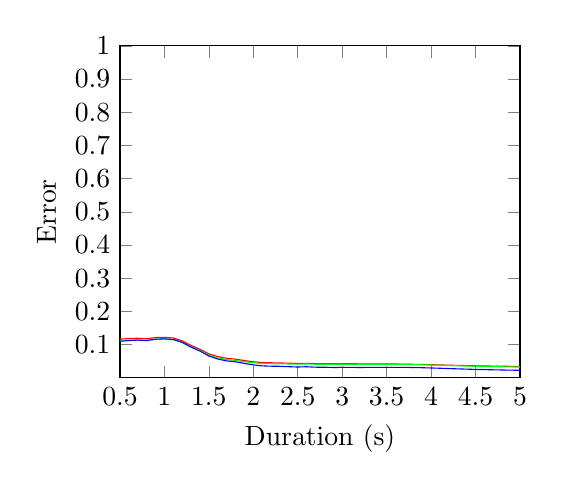
\begin{tikzpicture}

\begin{axis}[%
width= 2in,
height=1.66in,
at={(1.748842in,1.091895in)},
scale only axis,
xmin=0.5,
xmax=5,
xlabel={Duration (s)},
ytick={0.1,0.2,...,1,1.1},
xtick={0.5,1,...,4.5,5},
ymin=0,
ymax=1,
ylabel={Error},
title style={font=\bfseries},
legend style={legend cell align=left,align=left,draw=white!15!black}
]
\addplot [color=red,solid]
  table[row sep=crcr]{%
0.5	0.116606715060191\\
0.6	0.117997055105133\\
0.7	0.119102709903974\\
0.8	0.117525570741536\\
0.9	0.121125787159952\\
1	0.121848799026204\\
1.1	0.119844768728282\\
1.2	0.111293176404192\\
1.3	0.0972441692016664\\
1.4	0.0859201217596782\\
1.5	0.0719646971135904\\
1.6	0.0637925808506565\\
1.7	0.0587015571115359\\
1.8	0.056129189693083\\
1.9	0.0517798779009592\\
2	0.0482428904558047\\
2.1	0.0459797767399953\\
2.2	0.0451793517777765\\
2.3	0.0447058868379019\\
2.4	0.0438928826447229\\
2.5	0.0432485444401573\\
2.6	0.0435265998149818\\
2.7	0.0427019585418582\\
2.8	0.0426023542762414\\
2.9	0.0422630060176831\\
3	0.0422846181084555\\
3.1	0.0423041821959344\\
3.2	0.0420313721723238\\
3.3	0.0420868715251723\\
3.4	0.041845126835783\\
3.5	0.0417458915459075\\
3.6	0.0414308377400679\\
3.7	0.0411605921677774\\
3.8	0.0406069606036085\\
3.9	0.040013333767894\\
4	0.0393799772584942\\
4.1	0.0386907117981665\\
4.2	0.0379690145312799\\
4.3	0.0372910309735248\\
4.4	0.0366612662345494\\
4.5	0.036128938670861\\
4.6	0.035643285428503\\
4.7	0.0352075823255911\\
4.8	0.0347925486691523\\
4.9	0.0343939177741983\\
5	0.0341009792987977\\
};

%% \addlegendentry{\textbar bias\textbar=0};
\addplot [color=green,solid]
  table[row sep=crcr]{%
0.5	0.111629840333276\\
0.6	0.112941864217596\\
0.7	0.113999807359034\\
0.8	0.112401380716064\\
0.9	0.116039605389351\\
1	0.116821828487753\\
1.1	0.114901886148879\\
1.2	0.106446823821964\\
1.3	0.0925020301438534\\
1.4	0.081328558321378\\
1.5	0.0675516306037404\\
1.6	0.0595873966546359\\
1.7	0.0546893379224739\\
1.8	0.05233537519754\\
1.9	0.0482654296101405\\
2	0.0450379587938784\\
2.1	0.0430548359597281\\
2.2	0.0424590786680326\\
2.3	0.0421947777391173\\
2.4	0.0415724003923388\\
2.5	0.0411086546402141\\
2.6	0.0414965285365714\\
2.7	0.04085355568415\\
2.8	0.0408900976173342\\
2.9	0.0406790980406572\\
3	0.0408023651753037\\
3.1	0.040898540448454\\
3.2	0.0407386835119184\\
3.3	0.0408856900140973\\
3.4	0.0407055325787586\\
3.5	0.0406650688348556\\
3.6	0.0404025123480414\\
3.7	0.0401733262397001\\
3.8	0.0396314916571967\\
3.9	0.0390295938996\\
4	0.0383633615268031\\
4.1	0.0376379818458523\\
4.2	0.0368568157558358\\
4.3	0.0361050422745377\\
4.4	0.0354024030978923\\
4.5	0.0347817174123263\\
4.6	0.0342101140609905\\
4.7	0.033689405446034\\
4.8	0.0331949095418029\\
4.9	0.0327254959480877\\
5	0.0323533125743179\\
};
%% \addlegendentry{\textbar bias\textbar=0.05};

\addplot [color=blue,solid]
  table[row sep=crcr]{%
0.5	0.110205400460866\\
0.6	0.112059900874519\\
0.7	0.113445719597403\\
0.8	0.112196475852541\\
0.9	0.116185877950009\\
1	0.117178160150115\\
1.1	0.11540696886235\\
1.2	0.106864098599073\\
1.3	0.0923154592425234\\
1.4	0.0805508028389122\\
1.5	0.065674696763059\\
1.6	0.0565667683528162\\
1.7	0.0508590366634676\\
1.8	0.0481998958516259\\
1.9	0.0431166259404963\\
2	0.038744369905904\\
2.1	0.0358755619489716\\
2.2	0.0349167873159606\\
2.3	0.0345441744362363\\
2.4	0.0333996497756916\\
2.5	0.0324446398493226\\
2.6	0.0332340318487519\\
2.7	0.0319130081585281\\
2.8	0.0317762965859852\\
2.9	0.0310083577332042\\
3	0.0312478312313894\\
3.1	0.0313936412022642\\
3.2	0.030907768925086\\
3.3	0.0314917173744273\\
3.4	0.0311995738137807\\
3.5	0.031473719274027\\
3.6	0.031363804975408\\
3.7	0.0314509194095001\\
3.8	0.0309137299278705\\
3.9	0.0303162604615932\\
4	0.029549362213877\\
4.1	0.0287510007535127\\
4.2	0.027765935199653\\
4.3	0.0268347945146144\\
4.4	0.0260330332508285\\
4.5	0.0252621868822711\\
4.6	0.0246041161786416\\
4.7	0.0240225065899942\\
4.8	0.023483896835938\\
4.9	0.0229749792550578\\
5	0.0225526570431922\\
};
%% \addlegendentry{\textbar bias\textbar=0.2};

\end{axis}
\end{tikzpicture}%
}
                \caption{Gravity estimation error}

        \end{subfigure}%
        ~ %add desired spacing between images, e. g. ~, \quad, \qquad, \hfill etc.
          %(or a blank line to force the subfigure onto a new line)
        \begin{subfigure}[b]{0.5\columnwidth}
                \resizebox{\columnwidth}{!}{% This file was created by matlab2tikz.
% Minimal pgfplots version: 1.3
%
%The latest updates can be retrieved from
%  http://www.mathworks.com/matlabcentral/fileexchange/22022-matlab2tikz
%where you can also make suggestions and rate matlab2tikz.
%
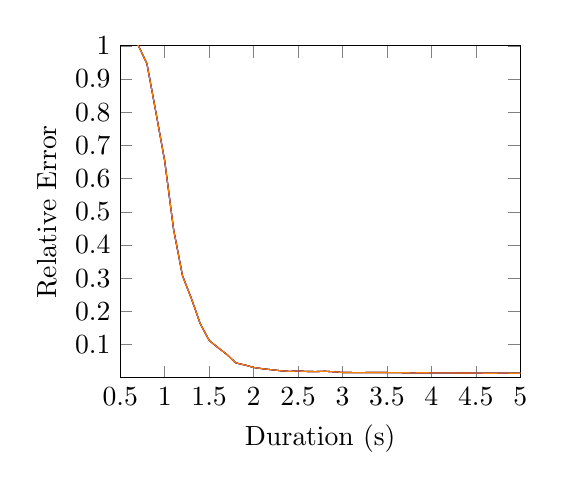
\begin{tikzpicture}

\begin{axis}[%
width= 2in,
height=1.66in,
at={(1.751579in,1.09421in)},
scale only axis,
xmin=0.5,
xmax=5,
xlabel={Duration (s)},
ytick={0.1,0.2,...,1,1.1},
xtick={0.5,1,...,4.5,5},
ymin=0,
ymax=1,
ylabel={Relative Error},
title style={font=\bfseries},
legend style={legend cell align=left,align=left,draw=white!15!black}
  ]
\addplot [color=red,solid]
  table[row sep=crcr]{%
0.5	1.03985490942799\\
0.6	1.041598565655\\
0.7	1.00236650429721\\
0.8	0.946285206056902\\
0.9	0.801144005638605\\
1	0.653111424622228\\
1.1	0.446952652972\\
1.2	0.307545014749713\\
1.3	0.238764359391316\\
1.4	0.162775041374018\\
1.5	0.112552620250376\\
1.6	0.0906560408733978\\
1.7	0.0702325874714304\\
1.8	0.0448237845321961\\
1.9	0.0386534542271255\\
2	0.0311057395082368\\
2.1	0.027271305531551\\
2.2	0.0242870145505906\\
2.3	0.0213446569284375\\
2.4	0.019253423110833\\
2.5	0.0202639766987494\\
2.6	0.0190928884123492\\
2.7	0.0186673514534201\\
2.8	0.0196889505362513\\
2.9	0.0181422306527873\\
3	0.0159381584340546\\
3.1	0.0157920847297511\\
3.2	0.0154584974482486\\
3.3	0.015976038710748\\
3.4	0.0158808936479735\\
3.5	0.0157693091644158\\
3.6	0.0156439004935535\\
3.7	0.0151820539225519\\
3.8	0.0148957930996785\\
3.9	0.0153153750167038\\
4	0.014933953322141\\
4.1	0.0146764838709416\\
4.2	0.0147039369508963\\
4.3	0.0142241103735529\\
4.4	0.0144684009758614\\
4.5	0.0140030229426442\\
4.6	0.0138009121378266\\
4.7	0.0137979864770686\\
4.8	0.0138945374601937\\
4.9	0.0138179103318856\\
5	0.0136531794141864\\
  };

\addplot [color=green,solid]
  table[row sep=crcr]{%
0.5	1.03985958098901\\
0.6	1.04160318355915\\
0.7	1.00237106009902\\
0.8	0.946289717389913\\
0.9	0.801148482808236\\
1	0.653115835094683\\
1.1	0.446956963215328\\
1.2	0.307549193614189\\
1.3	0.238768402671388\\
1.4	0.162778866000266\\
1.5	0.112556164989696\\
1.6	0.0906594511027657\\
1.7	0.0702357530206231\\
1.8	0.0448262850837141\\
1.9	0.0386556163799586\\
2	0.0311072877769502\\
2.1	0.0272723706785286\\
2.2	0.0242875971735912\\
2.3	0.0213446348227341\\
2.4	0.0192528393894945\\
2.5	0.0202634686746629\\
2.6	0.0190921269501307\\
2.7	0.0186664007188528\\
2.8	0.0196879239235448\\
2.9	0.0181410206611039\\
3	0.0159368124813167\\
3.1	0.0157906956206664\\
3.2	0.0154572915599915\\
3.3	0.015974943255289\\
3.4	0.0158797897599564\\
3.5	0.0157684278283326\\
3.6	0.0156430872283733\\
3.7	0.0151814885198358\\
3.8	0.014895146078053\\
3.9	0.0153144793914982\\
4	0.0149330818265368\\
4.1	0.0146758551046747\\
4.2	0.0147033461899024\\
4.3	0.0142233401735353\\
4.4	0.0144675984784877\\
4.5	0.0140021327931907\\
4.6	0.0138000012779865\\
4.7	0.0137971317684698\\
4.8	0.0138936794965301\\
4.9	0.0138170217044604\\
5	0.0136522219455462\\
  };

\addplot [color=blue,solid]
  table[row sep=crcr]{%
0.5	1.03986425207895\\
0.6	1.04160780091446\\
0.7	1.00237561027151\\
0.8	0.946294222676901\\
0.9	0.801152949003822\\
1	0.653120236997524\\
1.1	0.446961263559742\\
1.2	0.307553365956837\\
1.3	0.238772442420924\\
1.4	0.162782689585394\\
1.5	0.112559710919862\\
1.6	0.0906628620508701\\
1.7	0.0702389182838786\\
1.8	0.0448287832679672\\
1.9	0.0386577757661939\\
2	0.0311088319409189\\
2.1	0.0272734304054249\\
2.2	0.0242881740428105\\
2.3	0.0213446052217924\\
2.4	0.0192522476329966\\
2.5	0.0202629559685031\\
2.6	0.0190913614801648\\
2.7	0.0186654480077921\\
2.8	0.0196868997231422\\
2.9	0.0181398119199815\\
3	0.0159354608914177\\
3.1	0.0157892997710918\\
3.2	0.015456077806116\\
3.3	0.01597383905107\\
3.4	0.0158786758680475\\
3.5	0.0157675355582793\\
3.6	0.0156422624238909\\
3.7	0.0151809113268135\\
3.8	0.0148944876096839\\
3.9	0.0153135721746979\\
4	0.0149321986923262\\
4.1	0.0146752151128445\\
4.2	0.0147027437569585\\
4.3	0.0142225582675433\\
4.4	0.0144667839076757\\
4.5	0.014001231209046\\
4.6	0.0137990789502391\\
4.7	0.0137962654346151\\
4.8	0.0138928097441045\\
4.9	0.0138161214008475\\
5	0.0136512527044398\\
  };

\addplot [color=violet,solid]
  table[row sep=crcr]{%
0.5	1.03990162657298\\
0.6	1.04164474499346\\
0.7	1.00241202605313\\
0.8	0.946330255505779\\
0.9	0.801188651450575\\
1	0.653155418577664\\
1.1	0.44699564265194\\
1.2	0.307586738342365\\
1.3	0.238804769430305\\
1.4	0.162813294486986\\
1.5	0.112588099592512\\
1.6	0.0906901780032391\\
1.7	0.0702642726824345\\
1.8	0.0448488150337778\\
1.9	0.0386750988110832\\
2	0.0311212462405861\\
2.1	0.0272819801300415\\
2.2	0.0242928691246088\\
2.3	0.0213444647144645\\
2.4	0.0192476184012775\\
2.5	0.0202589351236235\\
2.6	0.0190853167280258\\
2.7	0.0186578952976754\\
2.8	0.019678747951536\\
2.9	0.0181301988233346\\
3	0.0159247584460048\\
3.1	0.0157782557374192\\
3.2	0.0154465046811283\\
3.3	0.0159651499258818\\
3.4	0.0158699220172952\\
3.5	0.0157605641007467\\
3.6	0.0156358378887817\\
3.7	0.0151764725213243\\
3.8	0.0148894013626436\\
3.9	0.0153064978034355\\
4	0.0149253210350167\\
4.1	0.0146702818693963\\
4.2	0.0146981137461654\\
4.3	0.0142164986112002\\
4.4	0.0144604637985282\\
4.5	0.0139942166176036\\
4.6	0.0137919001856516\\
4.7	0.0137895344889111\\
4.8	0.0138860507471762\\
4.9	0.0138091176101833\\
5	0.0136436989435932\\
  };

\addplot [color=orange,solid]
  table[row sep=crcr]{%
0.5	1.0399483433515\\
0.6	1.04169092245013\\
0.7	1.00245754542336\\
0.8	0.946375306304471\\
0.9	0.801233300755678\\
1	0.65319942001106\\
1.1	0.447038642504946\\
1.2	0.307628474533131\\
1.3	0.238845193954841\\
1.4	0.162851572957107\\
1.5	0.112623619899911\\
1.6	0.0907243680947724\\
1.7	0.0702960220793722\\
1.8	0.0448739356682219\\
1.9	0.0386968432854359\\
2	0.031136873332547\\
2.1	0.0272927883706028\\
2.2	0.0242988703409776\\
2.3	0.021344435140119\\
2.4	0.0192419882631464\\
2.5	0.0202540553915376\\
2.6	0.019077913510439\\
2.7	0.018648608793286\\
2.8	0.01966870426995\\
2.9	0.0181183393990501\\
3	0.015911557573295\\
3.1	0.015764629585974\\
3.2	0.0154347246807435\\
3.3	0.0159544706566606\\
3.4	0.0158591630136393\\
3.5	0.0157520374104561\\
3.6	0.0156279970977605\\
3.7	0.0151711224971348\\
3.8	0.0148832452227136\\
3.9	0.0152978479177686\\
4	0.0149169231583479\\
4.1	0.0146643221623784\\
4.2	0.0146925342577677\\
4.3	0.014209138691543\\
4.4	0.014452775411792\\
4.5	0.0139856678843345\\
4.6	0.01378315079938\\
4.7	0.0137813471009242\\
4.8	0.013877827820372\\
4.9	0.0138005907812756\\
5	0.0136344876929685\\
  };

\end{axis}
\end{tikzpicture}%
}
                \caption{Velocity estimation error}

        \end{subfigure}
        ~ %add desired spacing between images, e. g. ~, \quad, \qquad, \hfill etc.
          %(or a blank line to force the subfigure onto a new line)
        \begin{subfigure}[b]{0.5\columnwidth}
                \resizebox{\columnwidth}{!}{% This file was created by matlab2tikz.
% Minimal pgfplots version: 1.3
%
%The latest updates can be retrieved from
%  http://www.mathworks.com/matlabcentral/fileexchange/22022-matlab2tikz
%where you can also make suggestions and rate matlab2tikz.
%
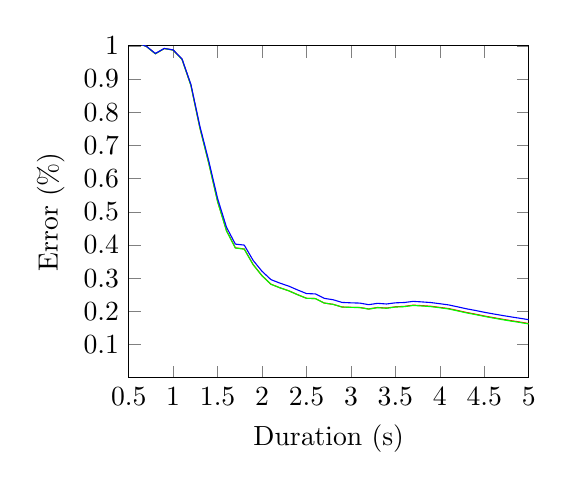
\begin{tikzpicture}

\begin{axis}[%
width= 2in,
height=1.66in,
at={(1.751579in,1.09421in)},
scale only axis,
xmin=0.5,
xmax=5,
xlabel={Duration (s)},
ytick={0.1,0.2,...,1,1.1},
xtick={0.5,1,...,4.5,5},
ymin=0,
ymax=1,
ylabel={Error (\%)},
title style={font=\bfseries},
legend style={legend cell align=left,align=left,draw=white!15!black}
  ]
  \addplot [color=red,solid]
  table[row sep=crcr]{%
0.5	1.00951410530102\\
0.6	1.00786500727994\\
0.7	0.997963442196014\\
0.8	0.976022633435467\\
0.9	0.991735794841291\\
1	0.987171007070719\\
1.1	0.959191161174873\\
1.2	0.880559973597208\\
1.3	0.753599673508593\\
1.4	0.64714017394003\\
1.5	0.531125453176089\\
1.6	0.443292785061992\\
1.7	0.391395148282084\\
1.8	0.387977686885945\\
1.9	0.340987973867047\\
2	0.307518122043313\\
2.1	0.281951244626588\\
2.2	0.271266589472539\\
2.3	0.262115154213078\\
2.4	0.250318101367763\\
2.5	0.239472046423177\\
2.6	0.238606700826374\\
2.7	0.225208554653766\\
2.8	0.221178376147107\\
2.9	0.213231764909724\\
3	0.212309557306614\\
3.1	0.211785233511893\\
3.2	0.207271207293066\\
3.3	0.211743350300891\\
3.4	0.210007717938161\\
3.5	0.213804710828916\\
3.6	0.215073807003346\\
3.7	0.21874238367089\\
3.8	0.217285974054173\\
3.9	0.215429772692012\\
4	0.212053995066442\\
4.1	0.20842968669488\\
4.2	0.202662265588549\\
4.3	0.19671514324955\\
4.4	0.191677465957092\\
4.5	0.186171819878279\\
4.6	0.181261579522324\\
4.7	0.176586227491708\\
4.8	0.172092653472152\\
4.9	0.167921896116196\\
5	0.163437045522267\\
};
%% \addlegendentry{\textbar bias\textbar=0};

\addplot [color=green,solid]
  table[row sep=crcr]{%
0.5	1.0094776108686\\
0.6	1.00782046331331\\
0.7	0.997859195886525\\
0.8	0.97585757944521\\
0.9	0.991648013616503\\
1	0.987064000499093\\
1.1	0.959028156661523\\
1.2	0.8802947972482\\
1.3	0.753225529356492\\
1.4	0.646680068394783\\
1.5	0.53057853917087\\
1.6	0.442726754472745\\
1.7	0.3908576649008\\
1.8	0.387499281479228\\
1.9	0.340552711374466\\
2	0.307138073630689\\
2.1	0.281641949028866\\
2.2	0.271038338318004\\
2.3	0.261958003737148\\
2.4	0.250215511813015\\
2.5	0.239403205097738\\
2.6	0.238557669558788\\
2.7	0.225140500957419\\
2.8	0.221075221903312\\
2.9	0.21306681345561\\
3	0.212068542828588\\
3.1	0.21145275411161\\
3.2	0.206830171767201\\
3.3	0.211195917371631\\
3.4	0.209346739493264\\
3.5	0.213040552079869\\
3.6	0.214213317362311\\
3.7	0.217798302526419\\
3.8	0.216266176372505\\
3.9	0.214345831750647\\
4	0.210916060777881\\
4.1	0.20725169651796\\
4.2	0.201451913806443\\
4.3	0.195481464349318\\
4.4	0.19042994398307\\
4.5	0.184914739496367\\
4.6	0.180000864130742\\
4.7	0.175325249431816\\
4.8	0.170833719417712\\
4.9	0.166666428729461\\
5	0.162183691340418\\
};
%% \addlegendentry{\textbar bias\textbar=0.05};

  \addplot [color=blue,solid]
  table[row sep=crcr]{%
0.5	1.0093654386579\\
0.6	1.00777216379647\\
0.7	0.998230278624944\\
0.8	0.976852811925765\\
0.9	0.991989950397821\\
1	0.987570683106742\\
1.1	0.960349030488607\\
1.2	0.883368764973945\\
1.3	0.758472463532796\\
1.4	0.653868010320715\\
1.5	0.540127936469423\\
1.6	0.453573542788974\\
1.7	0.402627589782717\\
1.8	0.39965705999988\\
1.9	0.353479790641683\\
2	0.320751349782662\\
2.1	0.295693651994372\\
2.2	0.285224497412259\\
2.3	0.276139475722294\\
2.4	0.264498941613126\\
2.5	0.253713745722727\\
2.6	0.252609370417162\\
2.7	0.239234372017261\\
2.8	0.235038093514646\\
2.9	0.226992160944722\\
3	0.225771519989974\\
3.1	0.224958566929275\\
3.2	0.22021014979355\\
3.3	0.224276315198198\\
3.4	0.222287103982913\\
3.5	0.225749113442478\\
3.6	0.22674696054832\\
3.7	0.23014720508112\\
3.8	0.228532688847528\\
3.9	0.226558330703094\\
4	0.223124383227352\\
4.1	0.21946057321155\\
4.2	0.213707978916598\\
4.3	0.207796950654789\\
4.4	0.20279668374678\\
4.5	0.197353401533552\\
4.6	0.1925013332922\\
4.7	0.187886267577429\\
4.8	0.18345141824562\\
4.9	0.179336350105221\\
5	0.174925096616426\\
};
%% \addlegendentry{\textbar bias\textbar=0.2};

\end{axis}
\end{tikzpicture}%
}
                \caption{Lambda estimation error}

        \end{subfigure}
        \caption{Impact of the accelerometer bias on the performance of the closed-form solution. We are observing 7 features  over a variable duration of integration.\label{fig:biasAccCF}}
\end{figure}

As seen on the Fig. \ref{fig:biasAccCF}, neither the gravity, the velocity or the lambdas are impacted by the accelerometer bias.

In \cite{Martinelli2014}, the author provides an alternative formulation of the closed-form solution including the accelerometer bias as an observable unknown of the system.
However, the estimation of the accelerometer bias with this method is not robust since our system is only slightly affected by it.

This is a counterintuitive results. Since our equations contain an integration of the acceleration, we also perform an integration of the accelerometer bias.
We would have expected the accelerometer bias to have a greater impact on the solutions yielded by the system.



\subsection{Impact of gyroscope bias on the performance}
Again, in order to visualize the impact of the gyroscope bias on the performance,
we corrupt the gyroscope measurements provided by our terrain IMU by adding an artificial bias (Fig. \ref{fig:biasGyroCF}).

Our experiments have shown that the presence of gyroscope bias significantly damages the results of the closed-form solution.

\begin{figure}[h!]
        \centering

        \begin{subfigure}[b]{0.5\columnwidth}
                \resizebox{\columnwidth}{!}{% This file was created by matlab2tikz.
% Minimal pgfplots version: 1.3
%
%The latest updates can be retrieved from
%  http://www.mathworks.com/matlabcentral/fileexchange/22022-matlab2tikz
%where you can also make suggestions and rate matlab2tikz.
%
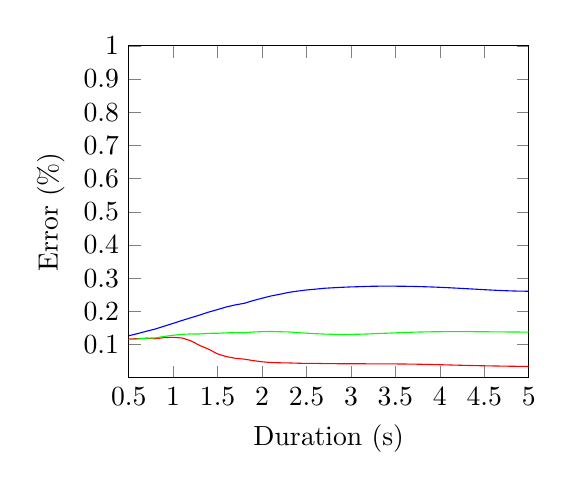
\begin{tikzpicture}

\begin{axis}[%
width= 2in,
height=1.66in,
at={(0.873053in,1.091895in)},
scale only axis,
xmin=0.5,
xmax=5,
xlabel={Duration (s)},
ytick={0.1,0.2,...,1,1.1},
xtick={0.5,1,...,4.5,5},
ymin=0,
ymax=1,
ylabel={Error (\%)},
title style={font=\bfseries},
legend style={legend cell align=left,align=left,draw=white!15!black}
]
\addplot [color=red,solid]
  table[row sep=crcr]{%
0.5	0.116606715060191\\
0.6	0.117997055105133\\
0.7	0.119102709903974\\
0.8	0.117525570741536\\
0.9	0.121125787159952\\
1	0.121848799026204\\
1.1	0.119844768728282\\
1.2	0.111293176404192\\
1.3	0.0972441692016664\\
1.4	0.0859201217596782\\
1.5	0.0719646971135904\\
1.6	0.0637925808506565\\
1.7	0.0587015571115359\\
1.8	0.056129189693083\\
1.9	0.0517798779009592\\
2	0.0482428904558047\\
2.1	0.0459797767399953\\
2.2	0.0451793517777765\\
2.3	0.0447058868379019\\
2.4	0.0438928826447229\\
2.5	0.0432485444401573\\
2.6	0.0435265998149818\\
2.7	0.0427019585418582\\
2.8	0.0426023542762414\\
2.9	0.0422630060176831\\
3	0.0422846181084555\\
3.1	0.0423041821959344\\
3.2	0.0420313721723238\\
3.3	0.0420868715251723\\
3.4	0.041845126835783\\
3.5	0.0417458915459075\\
3.6	0.0414308377400679\\
3.7	0.0411605921677774\\
3.8	0.0406069606036085\\
3.9	0.040013333767894\\
4	0.0393799772584942\\
4.1	0.0386907117981665\\
4.2	0.0379690145312799\\
4.3	0.0372910309735248\\
4.4	0.0366612662345494\\
4.5	0.036128938670861\\
4.6	0.035643285428503\\
4.7	0.0352075823255911\\
4.8	0.0347925486691523\\
4.9	0.0343939177741983\\
5	0.0341009792987977\\
};

%% \addlegendentry{\textbar bias\textbar =0};

\addplot [color=green,solid]
  table[row sep=crcr]{%
0.5	0.114794687547566\\
0.6	0.116779562670337\\
0.7	0.119185926413267\\
0.8	0.120120531727668\\
0.9	0.124610537501479\\
1	0.128052587957767\\
1.1	0.130926249443556\\
1.2	0.132078989798618\\
1.3	0.13192738084419\\
1.4	0.133950631948478\\
1.5	0.13407339510689\\
1.6	0.135451152760844\\
1.7	0.135876030068171\\
1.8	0.135476169238146\\
1.9	0.137907159471493\\
2	0.139008951294816\\
2.1	0.139465057704968\\
2.2	0.138679837236883\\
2.3	0.138093777901368\\
2.4	0.136212293045122\\
2.5	0.134306983207276\\
2.6	0.132848519704814\\
2.7	0.131699711866214\\
2.8	0.130920639935682\\
2.9	0.130421144778009\\
3	0.13078357013329\\
3.1	0.131253433397877\\
3.2	0.132089254038683\\
3.3	0.133355246577893\\
3.4	0.134215771247405\\
3.5	0.135345848264681\\
3.6	0.136359990672705\\
3.7	0.13735842784796\\
3.8	0.138002328772655\\
3.9	0.138489998145827\\
4	0.138794692629325\\
4.1	0.139006466534816\\
4.2	0.139021487405358\\
4.3	0.138926226194958\\
4.4	0.138800619376313\\
4.5	0.138616410667534\\
4.6	0.138405101734246\\
4.7	0.138178913135068\\
4.8	0.137949251009142\\
4.9	0.137750866645688\\
5	0.137634226533832\\
};
%% \addlegendentry{\textbar bias\textbar =0.05};

\addplot [color=blue,solid]
  table[row sep=crcr]{%
0.5	0.126540731489485\\
0.6	0.133059738131836\\
0.7	0.140191754416727\\
0.8	0.146993315210864\\
0.9	0.155514639755021\\
1	0.163943481621357\\
1.1	0.172603931314876\\
1.2	0.180994199517491\\
1.3	0.188952369328098\\
1.4	0.197870605066536\\
1.5	0.205499151242719\\
1.6	0.213456391224108\\
1.7	0.219618286221541\\
1.8	0.224293131663155\\
1.9	0.232533006914849\\
2	0.239594926602202\\
2.1	0.246385580596315\\
2.2	0.251619874636628\\
2.3	0.257204117125385\\
2.4	0.26116409581935\\
2.5	0.264500898715111\\
2.6	0.266903237389395\\
2.7	0.26963606191249\\
2.8	0.271118335838816\\
2.9	0.272560083765427\\
3	0.27373393339939\\
3.1	0.27445990331874\\
3.2	0.275477563174396\\
3.3	0.275863566646588\\
3.4	0.276042083151684\\
3.5	0.275903152314242\\
3.6	0.27565649154562\\
3.7	0.275145916729527\\
3.8	0.274474577722157\\
3.9	0.273601323214602\\
4	0.272523860177769\\
4.1	0.271275440688065\\
4.2	0.269875684720536\\
4.3	0.268394660815776\\
4.4	0.26687737570394\\
4.5	0.265365118898912\\
4.6	0.263948120121799\\
4.7	0.262694142312051\\
4.8	0.261675381813738\\
4.9	0.260977458906844\\
5	0.260686548115178\\
};
%% \addlegendentry{\textbar bias\textbar =0.2};


\end{axis}
\end{tikzpicture}%
}
                \caption{Gravity estimation error}

        \end{subfigure}%
        ~ %add desired spacing between images, e. g. ~, \quad, \qquad, \hfill etc.
          %(or a blank line to force the subfigure onto a new line)
        \begin{subfigure}[b]{0.5\columnwidth}
                \resizebox{\columnwidth}{!}{% This file was created by matlab2tikz.
% Minimal pgfplots version: 1.3
%
%The latest updates can be retrieved from
%  http://www.mathworks.com/matlabcentral/fileexchange/22022-matlab2tikz
%where you can also make suggestions and rate matlab2tikz.
%
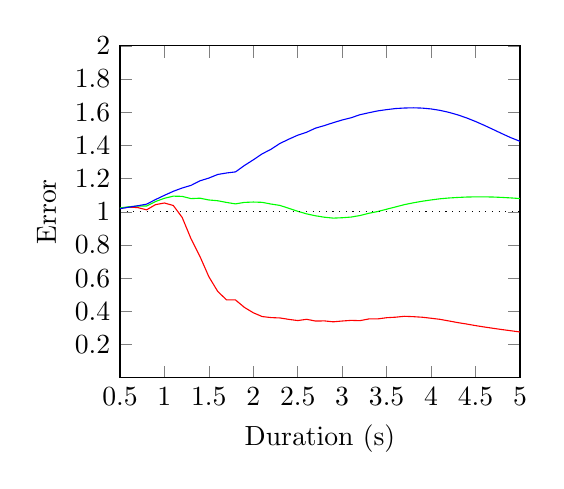
\begin{tikzpicture}

\begin{axis}[%
width= 2in,
height=1.66in,
at={(1.751579in,1.09421in)},
scale only axis,
unbounded coords=jump,
xmin=0.5,
xmax=5,
xlabel={Duration (s)},
ytick={0.2,0.4,...,1.8,2},
xtick={0.5,1,...,4.5,5},
ymin=0,
ymax=2,
ylabel={Error },
title style={font=\bfseries},
legend style={legend cell align=left,align=left,draw=white!15!black, at={(0.02,0.98)},anchor=north west}
]
\addplot [color=red,solid]
  table[row sep=crcr]{%
0.5	1.02175935565935\\
0.6	1.02791398584138\\
0.7	1.0256631041239\\
0.8	1.0119346333155\\
0.9	1.04321328865705\\
1	1.05305292291286\\
1.1	1.03815288783518\\
1.2	0.966235430882726\\
1.3	0.837047486448539\\
1.4	0.731229109725668\\
1.5	0.609284597782465\\
1.6	0.520318182824509\\
1.7	0.469135917702167\\
1.8	0.469085329131466\\
1.9	0.42429147636652\\
2	0.391855665299047\\
2.1	0.36905483808771\\
2.2	0.362779296792721\\
2.3	0.360542053306133\\
2.4	0.352030822201322\\
2.5	0.34487514314054\\
2.6	0.352486455310822\\
2.7	0.341992321163803\\
2.8	0.342831852614327\\
2.9	0.337300894873511\\
3	0.342135595088423\\
3.1	0.346018229140361\\
3.2	0.344320001070864\\
3.3	0.35468093595922\\
3.4	0.35488052155194\\
3.5	0.362036618911888\\
3.6	0.365160051746595\\
3.7	0.370578427179208\\
3.8	0.368363808036823\\
3.9	0.364986989708309\\
4	0.358867362407108\\
4.1	0.35230509491568\\
4.2	0.342589674214479\\
4.3	0.332678414221663\\
4.4	0.324003459162384\\
4.5	0.31454121832915\\
4.6	0.306091641043392\\
4.7	0.298130318170641\\
4.8	0.290540234885821\\
4.9	0.283328674546198\\
5	0.276133555094666\\
};
%% \addlegendentry{\textbar bias\textbar =0};

\addplot [color=green,solid]
  table[row sep=crcr]{%
0.5	1.02355207120059\\
0.6	1.03026860460552\\
0.7	1.03498841697354\\
0.8	1.03509865794458\\
0.9	1.06188179612969\\
1	1.08137067759546\\
1.1	1.09434528062304\\
1.2	1.09308614745031\\
1.3	1.07957133707453\\
1.4	1.08198629413277\\
1.5	1.07139175284461\\
1.6	1.06668737595967\\
1.7	1.0563822441038\\
1.8	1.04773112707274\\
1.9	1.05666989948084\\
2	1.05891389555878\\
2.1	1.05704076871567\\
2.2	1.04677684684384\\
2.3	1.0385257163595\\
2.4	1.02101065429131\\
2.5	1.00320585632867\\
2.6	0.987609688193366\\
2.7	0.976083363282641\\
2.8	0.967448011136072\\
2.9	0.961970778979797\\
3	0.964296165161102\\
3.1	0.968356703561008\\
3.2	0.977512329694832\\
3.3	0.991113113208863\\
3.4	1.00176372953356\\
3.5	1.0156246142103\\
3.6	1.02929430368843\\
3.7	1.04323363677726\\
3.8	1.05415319757685\\
3.9	1.06366706258245\\
4	1.07138552207739\\
4.1	1.07840513670921\\
4.2	1.08322640543848\\
4.3	1.0864422067885\\
4.4	1.08893879589077\\
4.5	1.0900916141486\\
4.6	1.0901160099761\\
4.7	1.08897843891426\\
4.8	1.08669231465207\\
4.9	1.08357561529757\\
5	1.07995032930589\\
};
%% \addlegendentry{\textbar bias\textbar =0.05};

\addplot [color=blue,solid]
  table[row sep=crcr]{%
0.5	1.01877763456232\\
0.6	1.0278748430534\\
0.7	1.03647684104063\\
0.8	1.04607509094039\\
0.9	1.07373182381123\\
1	1.0992378890232\\
1.1	1.12343639507097\\
1.2	1.14342836985361\\
1.3	1.15939843048576\\
1.4	1.18666195550943\\
1.5	1.20323355742176\\
1.6	1.22500916552771\\
1.7	1.23403164608103\\
1.8	1.24038676187243\\
1.9	1.27889382750531\\
2	1.31306054720695\\
2.1	1.34914949398501\\
2.2	1.37695229929848\\
2.3	1.41185295747137\\
2.4	1.43756656712845\\
2.5	1.46153871693893\\
2.6	1.47940128627451\\
2.7	1.50401782236624\\
2.8	1.5194677618903\\
2.9	1.5370086354038\\
3	1.55311037909986\\
3.1	1.56657245737693\\
3.2	1.58481513240264\\
3.3	1.59680156574203\\
3.4	1.6079711404209\\
3.5	1.61549676163322\\
3.6	1.62211616486494\\
3.7	1.62523473960433\\
3.8	1.62657662735924\\
3.9	1.62480370752791\\
4	1.61971926464314\\
4.1	1.61118324728822\\
4.2	1.59924533292031\\
4.3	1.584037537904\\
4.4	1.56559303673026\\
4.5	1.54422341843541\\
4.6	1.52064171983436\\
4.7	1.49566043709397\\
4.8	1.47029525716865\\
4.9	1.44602524985353\\
5	1.4247661626196\\
};
%% \addlegendentry{\textbar bias\textbar=0.2};

\draw[dotted] (axis cs:0.5,1) -- (axis cs:5,1);
%% \node at (axis cs:3.2,0.3) {\color{blue}\textbar bias\textbar=0.2 off chart};

\end{axis}
\end{tikzpicture}%
}
                \caption{Velocity estimation error}

        \end{subfigure}
        ~ %add desired spacing between images, e. g. ~, \quad, \qquad, \hfill etc.
          %(or a blank line to force the subfigure onto a new line)
        \begin{subfigure}[b]{0.5\columnwidth}
                \resizebox{\columnwidth}{!}{% This file was created by matlab2tikz.
% Minimal pgfplots version: 1.3
%
%The latest updates can be retrieved from
%  http://www.mathworks.com/matlabcentral/fileexchange/22022-matlab2tikz
%where you can also make suggestions and rate matlab2tikz.
%
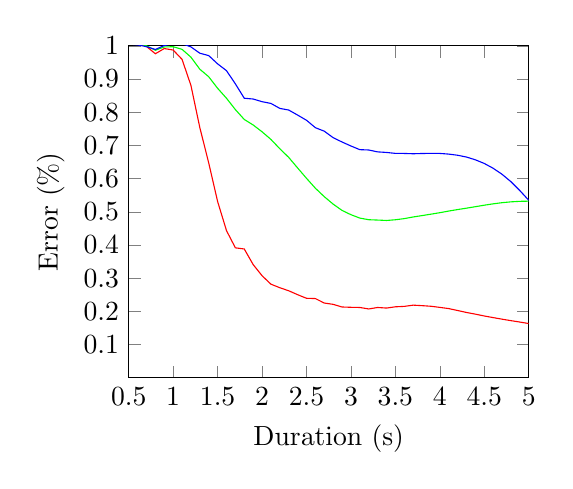
\begin{tikzpicture}

\begin{axis}[%
width= 2in,
height=1.66in,
at={(0.873053in,1.091895in)},
scale only axis,
xmin=0.5,
xmax=5,
xlabel={Duration (s)},
ytick={0.1,0.2,...,1,1.1},
xtick={0.5,1,...,4.5,5},
ymin=0,
ymax=1,
ylabel={Error (\%)},
title style={font=\bfseries},
legend style={legend cell align=left,align=left,draw=white!15!black, at={(0.02,0.02)},anchor=south west}
]
\addplot [color=red,solid]
  table[row sep=crcr]{%
0.5	1.00951410530102\\
0.6	1.00786500727994\\
0.7	0.997963442196014\\
0.8	0.976022633435467\\
0.9	0.991735794841291\\
1	0.987171007070719\\
1.1	0.959191161174873\\
1.2	0.880559973597208\\
1.3	0.753599673508593\\
1.4	0.64714017394003\\
1.5	0.531125453176089\\
1.6	0.443292785061992\\
1.7	0.391395148282084\\
1.8	0.387977686885945\\
1.9	0.340987973867047\\
2	0.307518122043313\\
2.1	0.281951244626588\\
2.2	0.271266589472539\\
2.3	0.262115154213078\\
2.4	0.250318101367763\\
2.5	0.239472046423177\\
2.6	0.238606700826374\\
2.7	0.225208554653766\\
2.8	0.221178376147107\\
2.9	0.213231764909724\\
3	0.212309557306614\\
3.1	0.211785233511893\\
3.2	0.207271207293066\\
3.3	0.211743350300891\\
3.4	0.210007717938161\\
3.5	0.213804710828916\\
3.6	0.215073807003346\\
3.7	0.21874238367089\\
3.8	0.217285974054173\\
3.9	0.215429772692012\\
4	0.212053995066442\\
4.1	0.20842968669488\\
4.2	0.202662265588549\\
4.3	0.19671514324955\\
4.4	0.191677465957092\\
4.5	0.186171819878279\\
4.6	0.181261579522324\\
4.7	0.176586227491708\\
4.8	0.172092653472152\\
4.9	0.167921896116196\\
5	0.163437045522267\\
};
%% \addlegendentry{\textbar bias\textbar =0};
\addplot [color=green,solid]
  table[row sep=crcr]{%
0.5	1.00976603989053\\
0.6	1.00662476967562\\
0.7	1.00012973781254\\
0.8	0.986574518220031\\
0.9	0.996468193911111\\
1	0.997191292079568\\
1.1	0.989272947419109\\
1.2	0.965751682085925\\
1.3	0.929424199744963\\
1.4	0.906767962367211\\
1.5	0.871992618329397\\
1.6	0.841943793167384\\
1.7	0.807821277321294\\
1.8	0.77807744676522\\
1.9	0.761474126867757\\
2	0.740961857659205\\
2.1	0.717953262447191\\
2.2	0.689879785205025\\
2.3	0.663803894329051\\
2.4	0.632095423347118\\
2.5	0.60084445997343\\
2.6	0.571000562078399\\
2.7	0.545538633038915\\
2.8	0.5230728282895\\
2.9	0.50414910231145\\
3	0.491242945800135\\
3.1	0.481064422015891\\
3.2	0.476101072394541\\
3.3	0.475079165506583\\
3.4	0.473811233300238\\
3.5	0.475983020538331\\
3.6	0.479418542197959\\
3.7	0.484363209456063\\
3.8	0.488507313989463\\
3.9	0.492844791089123\\
4	0.497216842204406\\
4.1	0.502169589937954\\
4.2	0.506688957686255\\
4.3	0.510885339429029\\
4.4	0.515377948688574\\
4.5	0.519860523702652\\
4.6	0.523924558142122\\
4.7	0.527385772041591\\
4.8	0.529917959141794\\
4.9	0.531484021602687\\
5	0.532017565178826\\
};
%% \addlegendentry{\textbar bias\textbar =0.05};

\addplot [color=blue,solid]
  table[row sep=crcr]{%
0.5	1.00524141035264\\
0.6	1.00274701979814\\
0.7	0.997268270597166\\
0.8	0.98888494572059\\
0.9	1.00083746170205\\
1	1.00647274030102\\
1.1	1.00643276611151\\
1.2	0.996650921332219\\
1.3	0.977579185243088\\
1.4	0.970454919162685\\
1.5	0.945587673080297\\
1.6	0.925094800347431\\
1.7	0.885263414803394\\
1.8	0.842031385070856\\
1.9	0.839647895258603\\
2	0.831641010373843\\
2.1	0.826371171011399\\
2.2	0.811393192785814\\
2.3	0.806467392158359\\
2.4	0.791354283346187\\
2.5	0.775653721210895\\
2.6	0.753330436822953\\
2.7	0.742740535205827\\
2.8	0.723242895764714\\
2.9	0.710193235407557\\
3	0.698171455279555\\
3.1	0.68714281385326\\
3.2	0.686124732881851\\
3.3	0.680430884015626\\
3.4	0.678731821158565\\
3.5	0.675918001322819\\
3.6	0.675706227822975\\
3.7	0.674803760488682\\
3.8	0.675568678230119\\
3.9	0.675956021801714\\
4	0.675744775832737\\
4.1	0.673765761159493\\
4.2	0.670295849423134\\
4.3	0.664866628301337\\
4.4	0.656566895248469\\
4.5	0.645544299301759\\
4.6	0.631084282882008\\
4.7	0.612963486493626\\
4.8	0.59059741833706\\
4.9	0.563876519376817\\
5	0.534843429135507\\
};
%% \addlegendentry{\textbar bias\textbar =0.2};



\end{axis}
\end{tikzpicture}%
}
                \caption{Lambda estimation error}

        \end{subfigure}
        \caption{Impact of the gyroscope bias on the performance of the closed-form solution. We are observing 7 features over a variable duration of integration. \label{fig:biasGyroCF}}
\end{figure}

As seen in Fig. \ref{fig:biasGyroCF}, the performance becomes very poor in presence of a bias on the gyroscope and, in practice, the overall method could only be successfully used with a very precise---and expensive---gyroscope.



\section{ESTIMATING THE GYROSCOPE BIAS}

Previous work has shown that the gyroscope bias is an observable mode when using an IMU and a camera, which means that it can be estimated \cite{Martinelli2012}.

Optimally, we would add the gyroscope bias in our unknown vector $X$ and determine $X$ by simply inverting the system $\Xi X = S$ as in the standard closed-form solution.
However, we can not express the gyroscope bias linearly with this system.

In this section, we propose a different approach to estimate the gyroscope bias using the closed-form solution.

\subsection{Nonlinear minimization of the residual}

Since our system of equations (\ref{eq:final1}) is overconstrained,
inverting it is equivalent to finding the vector $X$ that minimizes the residual $||\Xi X - S||^2$.

Since we can not express the gyroscope bias linearly,
we define the following cost function:

\begin{equation}
  \label{eq:cost}
  cost(B) = ||\Xi X - S||^2
\end{equation}

With:
\begin{itemize}
\item $B$ the gyroscope bias;
\item $\Xi$ and $S$ computed with respect to $B$.
\end{itemize}

By minimizing this cost function, we recover the gyroscope bias $B$ and the unknown vector $X$ which compensated for the gyroscope bias $B$.
We can initialize the optimization process with $B = 0_3$ since the bias is usually a rather small quantity.

\begin{figure}[h!]
  \centering
  \resizebox{0.7\columnwidth}{!}{% This file was created by matlab2tikz.
% Minimal pgfplots version: 1.3
%
%The latest updates can be retrieved from
%  http://www.mathworks.com/matlabcentral/fileexchange/22022-matlab2tikz
%where you can also make suggestions and rate matlab2tikz.
%
\definecolor{mycolor1}{rgb}{0.00000,0.44700,0.74100}%
%
\begin{tikzpicture}



\begin{axis}[%
width=4.6in,
height=1in,
at={(0in,3in)},
scale only axis,
xmin=1.5,
xmax=4.5,
xlabel={Duration (s)},
ytick={-0.05,0.0276,0.05},
ymin=-0.06,
ymax=0.06,
xtick={1.5, 2,...,4, 4.5},
ylabel={Bias (rad/s)}
]
\addplot [color=mycolor1,solid,forget plot]
  table[row sep=crcr]{%
1.91728659346996	0.072\\
2	0.0332103321872858\\
2.5	0.025037245454736\\
3	0.0321581893592385\\
3.5	0.027530467500012\\
4	0.0241138134913708\\
4.5	0.0280167461197849\\
};
\draw[line width=2pt,loosely dotted]  (1.5,0.0276 ) -- (4.5,0.0276);
\end{axis}


\begin{axis}[%
width=4.6in,
height=1in,
at={(0in,1.5in)},
scale only axis,
xmin=1.5,
xmax=4.5,
xlabel={Duration (s)},
ymin=-0.06,
ymax=0.06,
xtick={1.5, 2,...,4, 4.5},
ytick={-0.05,-0.0024,0.05},
ylabel={Bias (rad/s)}
]
\addplot [color=mycolor1,solid,forget plot]
  table[row sep=crcr]{%
1.73915180031747	-0.072\\
2	-0.00171936386040559\\
2.5	-0.00299882445661285\\
3	0.00306235287226103\\
3.5	-0.00341664285341729\\
4	-0.00756449922739225\\
4.5	-0.00255081057036582\\
};
\draw[line width=2pt,loosely dotted]  (1.5,-0.0024) -- (4.5,-0.0024);
\end{axis}

\begin{axis}[%
width=4.6in,
height=1in,
at={(0in,0in)},
scale only axis,
xmin=1.5,
xmax=4.5,
xlabel={Duration (s)},
ymin=-0.06,
ymax=0.06,
xtick={1.5, 2,...,4, 4.5},
ytick={-0.05,0.0417},
ylabel={ Bias (rad/s)}
]
\addplot [color=mycolor1,solid,forget plot]
  table[row sep=crcr]
  \caption{Gyroscope bias estimation from nonlinear minimization of the residual. We are observing 30 features  over a variable duration of integration. The true gyroscope bias is $[0.0276,   -0.0024,    0.0417]$. \label{fig:gBiasEstimate}}
\end{figure}

\begin{figure}[h!]
   \centering
   \resizebox{0.7\columnwidth}{!}{% This file was created by matlab2tikz.
% Minimal pgfplots version: 1.3
%
%The latest updates can be retrieved from
%  http://www.mathworks.com/matlabcentral/fileexchange/22022-matlab2tikz
%where you can also make suggestions and rate matlab2tikz.
%
\definecolor{mycolor1}{rgb}{0,1,0}%
%
\begin{tikzpicture}

\begin{axis}[%
width=4.5in,
height=3.7in,
at={(1.751579in,1.09421in)},
scale only axis,
xmin=1.5,
xmax=4.5,
xlabel={Duration (s)},
ytick={0.1,0.2,...,1,1.1},
xtick={1.5,2,...,4,4.5},
ymin=0,
ymax=1,
ylabel={Error},
%ylabel style={rotate=-90},
legend style={legend cell align=left,align=left,draw=white!15!black}
]

\addplot [color=blue,solid]
  table[row sep=crcr]{%
1.5	0.750383698320232\\
2	0.295866099048781\\
2.5	0.200527305989801\\
3	0.0764362409746096\\
3.5	0.100959038356456\\
4	0.0948731394402614\\
4.5	0.0798354774457304\\
};
\addlegendentry{lambda};

\addplot [color=red,solid]
  table[row sep=crcr]{%
1.5	0.974150779498911\\
2	0.605529789406788\\
2.5	0.518703606130607\\
3	0.317612029278896\\
3.5	0.282899391695432\\
4	0.292200875938786\\
4.5	0.364837441329439\\
};
\addlegendentry{speed};

\addplot [color=mycolor1,solid]
  table[row sep=crcr]{%
1.5	0.169913766671503\\
2	0.0945111315939618\\
2.5	0.0784139955620268\\
3	0.0450002320038315\\
3.5	0.0398138498948057\\
4	0.0425201881678023\\
4.5	0.0518673738017392\\
};
\addlegendentry{gravity};

\addplot [color=blue,dashed,forget plot]
  table[row sep=crcr]{%
1.5	1.00000695085483\\
2	0.121632544641259\\
2.5	0.0803545574381917\\
3	0.00633738663790857\\
3.5	0.0498493223835613\\
4	0.0649427778633683\\
4.5	0.0329546329957078\\
};
\addplot [color=red,dashed,forget plot]
  table[row sep=crcr]{%
1.5	1.01544354352349\\
2	0.28414184499176\\
2.5	0.235306474274456\\
3	0.273320881356479\\
3.5	0.23861115867277\\
4	0.211236751678519\\
4.5	0.232308133566351\\
};
\addplot [color=mycolor1,dashed,forget plot]
  table[row sep=crcr]
                \caption{Estimation error of the closed-form solution against the optimized closed-form solution.  We are observing 30 features  over a variable duration of integration. The true gyroscope bias is $[0.0276,   -0.0024,    0.0417]$. \label{fig:optEstimate}}
\end{figure}

\begin{figure}[h!]
        \centering

        \begin{subfigure}[b]{0.5\columnwidth}
                \resizebox{\columnwidth}{!}{% This file was created by matlab2tikz.
% Minimal pgfplots version: 1.3
%
%The latest updates can be retrieved from
%  http://www.mathworks.com/matlabcentral/fileexchange/22022-matlab2tikz
%where you can also make suggestions and rate matlab2tikz.
%
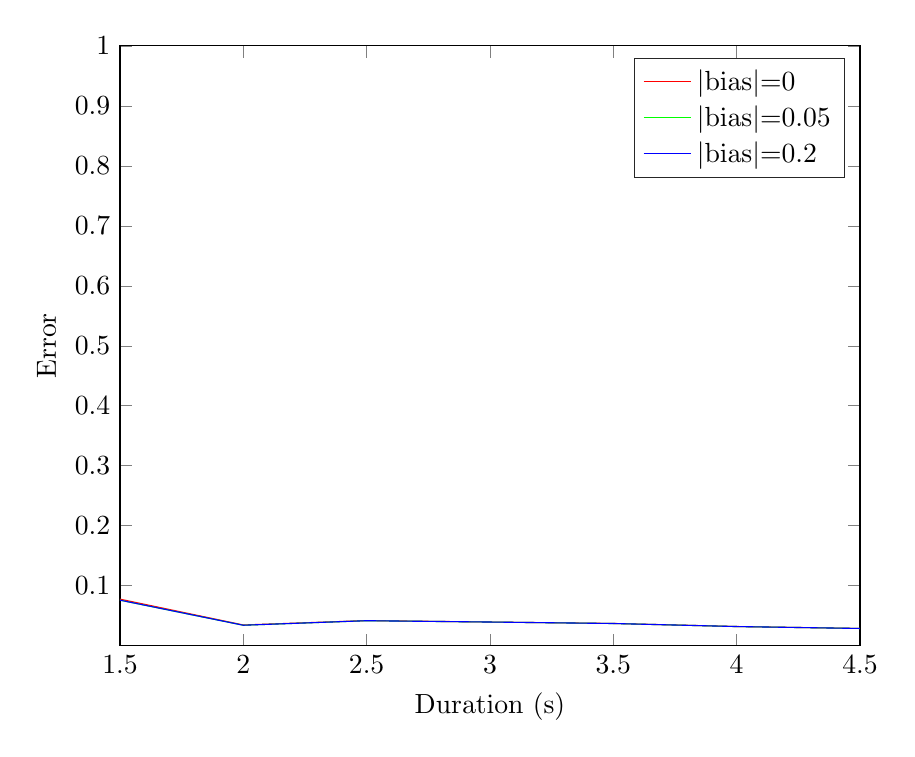
\begin{tikzpicture}

\begin{axis}[%
width=3.7in,
height=3in,
at={(1.748842in,1.091895in)},
scale only axis,
xmin=1.5,
xmax=4.5,
xlabel={Duration (s)},
ytick={0.1,0.2,...,1,1.1},
xtick={1.5,2,...,4,4.5},
ymin=0,
ymax=1,
ylabel={Error},
legend style={legend cell align=left,align=left,draw=white!15!black}
]
\addplot [color=red,solid]
  table[row sep=crcr]{%
1.5	0.0777063235422607\\
2	0.0346546036007086\\
2.5	0.0419789524726965\\
3	0.0395582076215153\\
3.5	0.0371856919479813\\
4	0.0320777150694178\\
4.5	0.0288476156134921\\
};
\addlegendentry{\textbar bias\textbar =0};

\addplot [color=green,solid]
  table[row sep=crcr]{%
1.5	0.0760217965122084\\
2	0.0342089064100465\\
2.5	0.0417690974320374\\
3	0.039548839289346\\
3.5	0.0370988331569301\\
4	0.0320211067326042\\
4.5	0.0288263176921808\\
};
\addlegendentry{\textbar bias\textbar =0.05};

\addplot [color=blue,solid]
  table[row sep=crcr]
                \caption{Gravity estimation relative error}

        \end{subfigure}%
        ~ %add desired spacing between images, e. g. ~, \quad, \qquad, \hfill etc.
          %(or a blank line to force the subfigure onto a new line)
        \begin{subfigure}[b]{0.5\columnwidth}
                \resizebox{\columnwidth}{!}{% This file was created by matlab2tikz.
% Minimal pgfplots version: 1.3
%
%The latest updates can be retrieved from
%  http://www.mathworks.com/matlabcentral/fileexchange/22022-matlab2tikz
%where you can also make suggestions and rate matlab2tikz.
%
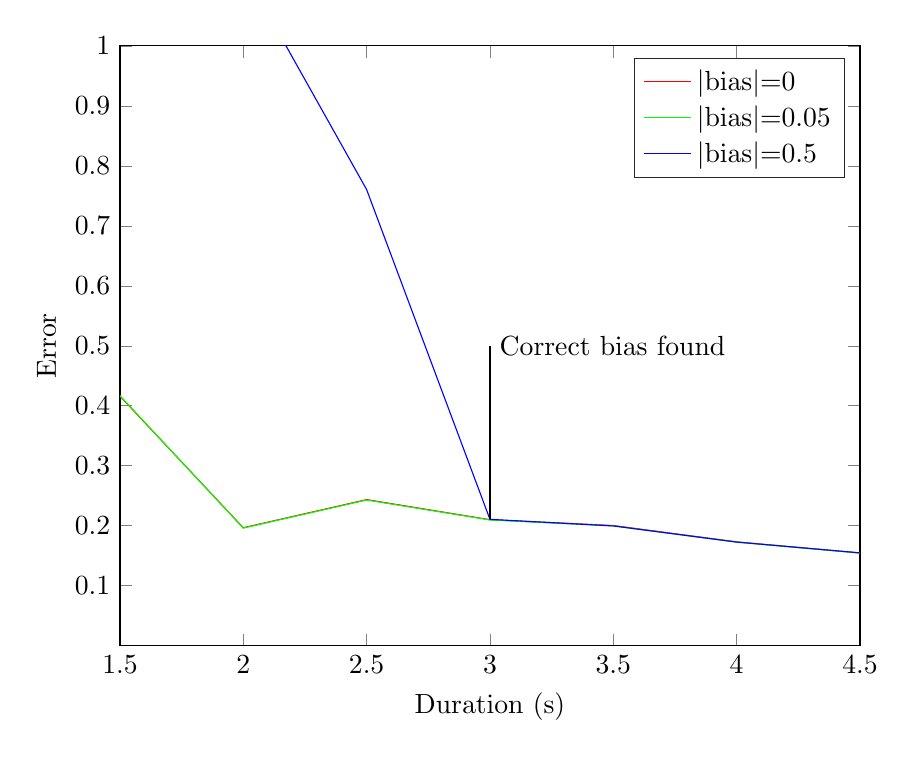
\begin{tikzpicture}

\begin{axis}[%
width=3.7in,
height=3in,
at={(1.751579in,1.09421in)},
scale only axis,
xmin=1.5,
xmax=4.5,
xlabel={Duration (s)},
ytick={0.1,0.2,...,1,1.1},
xtick={1.5,2,...,4,4.5},
ymin=0,
ymax=1,
ylabel={ Error},
legend style={legend cell align=left,align=left,draw=white!15!black}
]
\addplot [color=red,solid]
  table[row sep=crcr]{%
1.5	0.416014163169207\\
2	0.196683554909346\\
2.5	0.243582740699315\\
3	0.210126115008794\\
3.5	0.200403399493516\\
4	0.173117481975929\\
4.5	0.1547038991148\\
};
\addlegendentry{\textbar bias\textbar =0};

\addplot [color=green,solid]
  table[row sep=crcr]{%
1.5	0.41691124744351\\
2	0.196085518742207\\
2.5	0.242845859433578\\
3	0.209595541753857\\
3.5	0.199692504930268\\
4	0.172636924048922\\
4.5	0.154506893070617\\
};
\addlegendentry{\textbar bias\textbar =0.05};

\addplot [color=blue,solid]
  table[row sep=crcr]
                \caption{Velocity estimation relative error}

        \end{subfigure}
        ~ %add desired spacing between images, e. g. ~, \quad, \qquad, \hfill etc.
          %(or a blank line to force the subfigure onto a new line)
        \begin{subfigure}[b]{0.5\columnwidth}
                \resizebox{\columnwidth}{!}{% This file was created by matlab2tikz.
% Minimal pgfplots version: 1.3
%
%The latest updates can be retrieved from
%  http://www.mathworks.com/matlabcentral/fileexchange/22022-matlab2tikz
%where you can also make suggestions and rate matlab2tikz.
%
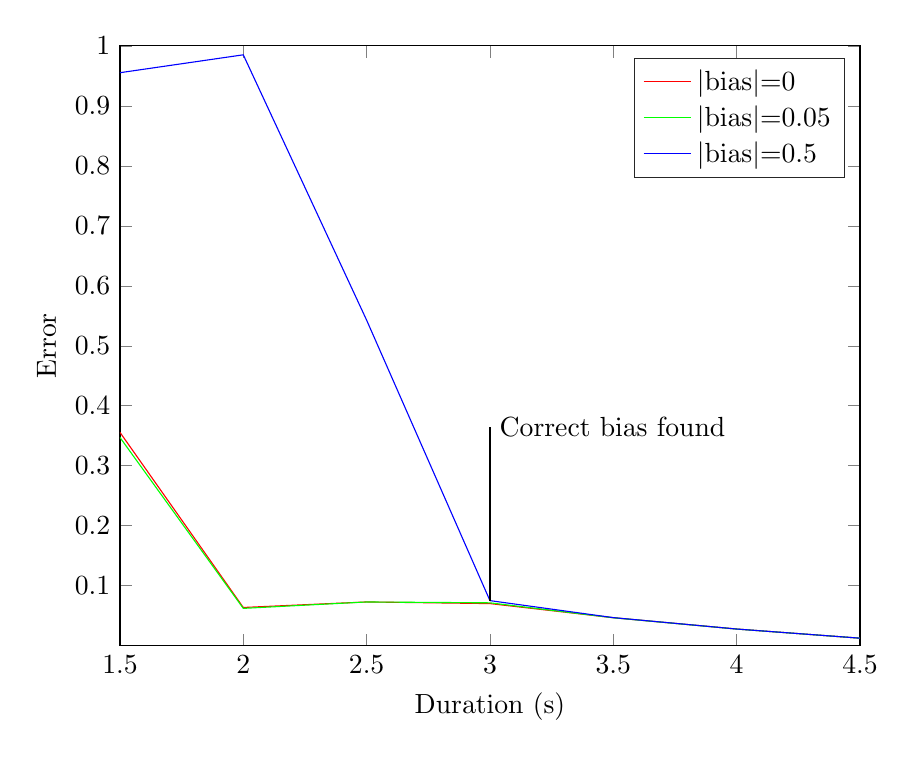
\begin{tikzpicture}

\begin{axis}[%
width=3.7in,
height=3in,
at={(1.751579in,1.09421in)},
scale only axis,
xmin=1.5,
xmax=4.5,
xlabel={Duration (s)},
ytick={0.1,0.2,...,1,1.1},
xtick={1.5,2,...,4,4.5},
ymin=0,
ymax=1,
ylabel={Error},
legend style={legend cell align=left,align=left,draw=white!15!black}
]
\addplot [color=red,solid]
  table[row sep=crcr]{%
1.5	0.355718720318707\\
2	0.0638186739379322\\
2.5	0.0730477252365667\\
3	0.0702721398950919\\
3.5	0.0467479539140586\\
4	0.0279088740708369\\
4.5	0.0126154029140042\\
};
\addlegendentry{\textbar bias\textbar =0};

\addplot [color=green,solid]
  table[row sep=crcr]{%
1.5	0.347243972870017\\
2	0.0623085495559465\\
2.5	0.0729871936167261\\
3	0.0715737368927602\\
3.5	0.0466612686519153\\
4	0.0278146137850077\\
4.5	0.0126401174100688\\
};
\addlegendentry{\textbar bias\textbar =0.05};

\addplot [color=blue,solid]
  table[row sep=crcr]
                \caption{Lambda estimation relative error}

        \end{subfigure}
        \caption{Impact of the gyroscope bias on the performance of the optimized closed-form solution. We are observing 7 features  over a variable duration of integration. \label{fig:biasGyroOpt}}
\end{figure}

%% This technique is similar to the one used in \cite{Abbeel2005}, where the author minimizes the residual of a Kalman filter in order to recover the noise matrix for the sensors.

The optimized closed-form solution provides better results than the standard closed-form solution. Fig. \ref{fig:optEstimate} depicts an improvement in precision of around $5\%$ for the distance to the features, and around $13\%$ for the speed after 4 seconds of integration.

Moreover, the optimized closed-form solution requires a shorter integration duration to provide good quality results.
Specifically, after 2 seconds of integration (around 7 camera observations) the provided estimations are already robust.
The non-optimized closed-form solution requires 3 seconds of integration before converging to acceptable estimations.


Lastly, this method is robust even for high values of the gyroscope bias.
Fig. \ref{fig:biasGyroOpt} represents the quality of the estimations with the same artificial gyroscope bias from Fig. \ref{fig:biasGyroCF}.



As seen in Fig. \ref{fig:biasGyroOpt}, after a certain integration duration, the estimations agree no matter how high the bias is.
Moreover, the values on which these evaluations agree are equals to the ones in Fig. \ref{fig:biasGyroCF} for the curve that has a gyroscope bias set to $0_3$.


By adding this new method for the bias estimation to the original method we obtain results which are equivalent to the ones in absence of bias.
Compared to the original method, the new method is now robust to the gyroscope bias, and also provides the gyroscope bias.

\section{VALIDATION}

We validate our method against a different dataset than the one we used in the previous sections to draw our conclusions.
Specifically, it contains IMU and camera measurements along with ground truth.
Therefore, we are now only relying on fully real terrain data,
but also we do not have the ground truth for the distance to the point features anymore.
The drone is flying indoor at low altitude.
The feature extraction and matching is done with FAST corner algrotihm as in \cite{Forster2014}.

We compare the performance on the estimations of the gravity and the initial velocity obtained with three different methods:
\begin{itemize}
\item The original closed-form solution (Equation \ref{eq:mat1});
\item Our modified closed-form solution (Equation \ref{eq:cost});
\item Fast Semi-Direct Monocular Visual Odometry (SVO) described in \cite{Forster2014}.
\end{itemize}
The reason we included the SVO in the validation is for having a reference to state of the art visual inertial fusion method.
However, this method requires to be initialized with the knowledge of the absolute scale.

We set the integration duration for the closed-form solution to 2 seconds.
The camera provides 60fps, but we discard most of the observations and consider only one observation every 0.3 seconds.
Indeed, adding observations that are too close to each other does not add significant information to our system.

%In a real applications, a proper online computation of the gyroscope bias can be reused.
%% Since the gyroscope bias varies slowly over time, we can reuse its knowledge.
%% In other words, we can use the optimized closed-form solution to compute the bias at the beginning of the sequence.
%% Thereafter, we can quickly provide reliable state estimations with the standard closed-form solution by compensating with the computed bias.

%% For long term navigation (longer than a minute), it would be advised to recompute the gyroscope bias every so often.
%% This re-computation can use the knowledge of previously computed bias. % as stated in Section \ref{sec:reg}.

%% The reason why we do not run the optimization for every state estimation is to speed up the computation.
%% Despite the optimization is relatively fast since our cost function is defined only with respect to the gyroscope bias, it still has to run the closed-form solution several times for its gradient descent to converge.
%% We found by experimentation that it usually requires around 6 iterations to converge.


\section{CONCLUSION}


\bibliographystyle{plain}
\bibliography{library}

\end{document}
